\documentclass[letterpaper]{article}
\usepackage{jair,balance}
\usepackage{times,helvet,courier}
\usepackage{amssymb,amsmath,amsthm,bm}
\usepackage[ruled, vlined,linesnumbered]{algorithm2e}
\usepackage{graphicx,multirow,array}
\usepackage{caption}
\usepackage{subcaption}
\usepackage{enumitem,pgfplots,fancyvrb}
\usepackage[output-decimal-marker={,},exponent-product=\cdot]{siunitx}
\usepackage{icomma}
\usepackage{amsmath}
\usepackage{rotating,color}


\SetKwFor{Loop}{Loop}{}{EndLoop}

\usepackage{tikz}
\usetikzlibrary{decorations.pathreplacing}
\pgfplotsset{compat=1.13}

\usepackage{todonotes}

\usepackage{pdfrender}

\def\memout{\hspace*{\fill}--\hspace*{\fill}}
\newcommand{\eg}{e.\,g.}
\newcommand{\ie}{i.\,e.}
\newtheorem{proposition}{Proposition}
\newtheorem{theorem}{Theorem}
\newtheorem{lemma}{Lemma}
\newtheorem{example}{Example}

\newtheoremstyle{my_def}% name
  {5pt}%      Space above
  {5pt}%      Space below
  {}%         Body font
  {}%         Indent amount (empty = no indent, \parindent = para indent)
  {\bfseries}% Thm head font
  {.}%        Punctuation after thm head
  {.5em}%     Space after thm head: " " = normal interword space;
        %       \newline = linebreak
  {{#1} {#2} (\thmnote{#3})}%         Thm head spec (can be left empty, meaning `normal')
\theoremstyle{my_def}
\newtheorem{definition}{Definition}

\newcommand{\astar}{\ensuremath{\textup{A}^*}}
\newcommand{\idastar}{\ensuremath{\textup{IDA}^*}}
\newcommand{\ha}{\ensuremath{\mathcal{H}}}

\newcommand{\R}{\ensuremath{\mathcal{R}}}
\newcommand{\var}{\ensuremath{\mathit{Var}}}
\newcommand{\loc}{\ensuremath{\mathit{Loc}}}
\newcommand{\relc}{\ensuremath{\mathit{Flow}}}
\newcommand{\reld}{\ensuremath{\mathit{Trans}}}
\newcommand{\inv}{\ensuremath{\mathit{I}}}
\newcommand{\Input}{\ensuremath{\mathcal{U}}}
\newcommand{\RealUniverse}{\ensuremath{\mathbb{R}^n}}
\newcommand{\update}{\ensuremath{\xi}}
\newcommand{\guard}{\ensuremath{g}}
\newcommand{\HyperBox}{\ensuremath{\mathcal{B}}}
\newcommand{\Vector}[1]{\ensuremath{\mathbf{#1}}}
\newcommand{\PostC}[2]{post_c(#1,#2)}
\newcommand{\PostD}[2]{post_d(#1,#2)}
\newcommand{\sync}{\ensuremath{\mathit{Sync}}}
\newcommand{\lab}{\ensuremath{\mathit{label}}}
\newcommand{\dur}{\ensuremath{\mathit{dur}}}
\newcommand{\lockstart}{\ensuremath{\overline{\mathit{lock}_a^\mathit{start}}}}
\newcommand{\lockend}{\ensuremath{\overline{\mathit{lock}_a^\mathit{end}}}}
\newcommand{\releasestart}{\ensuremath{\overline{\mathit{release}_a^\mathit{start}}}}
\newcommand{\releaseend}{\ensuremath{\overline{\mathit{release}_a^\mathit{end}}}}
\newcommand{\lock}{\ensuremath{\overline{\mathit{lock}_a}}}
\newcommand{\release}{\ensuremath{\overline{\mathit{release}_a}}}
\newcommand{\lockstartend}{\ensuremath{\overline{\mathit{lock}_a^\mathit{start/end}}}}
\newcommand{\releasestartend}{\ensuremath{\overline{\mathit{release}_a^\mathit{start/end}}}}

\newcommand{\ContState}{\mathbf{x}}
\newcommand{\ContStateFunc}{\mathbf{X}}
\newcommand{\DiscStateFunc}{L}
\newcommand{\ContStateStart}{\mathbf{X}_{start}}
\newcommand{\ContStateEnd}{\mathbf{X}_{end}}
\newcommand{\run}{\rho}
\newcommand{\traj}{\tau}

\newcommand{\network}{\ensuremath{\mathcal{N}}}
\renewcommand{\epsilon}{\ensuremath{\varepsilon}}

\newcommand{\dom}{\ensuremath{\mathit{Dom}}}
\newcommand{\prob}{\ensuremath{\mathit{Prob}}}
\newcommand{\fs}{\ensuremath{\mathit{Fs}}}
\newcommand{\rs}{\ensuremath{\mathit{Rs}}}
\newcommand{\as}{\ensuremath{\mathit{As}}}
\newcommand{\ps}{\ensuremath{\mathit{Ps}}}
\newcommand{\es}{\ensuremath{\mathit{Es}}}
\newcommand{\arity}{\ensuremath{\mathit{arity}}}
\newcommand{\os}{\ensuremath{\mathit{Os}}}
\newcommand{\init}{\ensuremath{\mathit{Init}}}
\newcommand{\Hinit}{\ensuremath{\mathit{Init}}}

\newcommand{\headingtimeaction}{{\bf Time} \qquad \= {\bf Action}\\[0.8ex]}
\newcommand{\headingtimehappening}{{\bf Time} \qquad \= {\bf Happening}\\[0.8ex]}
\newcommand{\headingtimedetails}{{\bf Time} \qquad \= {\bf Details}\\[0.8ex]}
\newcommand{\atime}[1]{{\bf #1:}}
\newcommand{\action}[1]{{\sf #1}}
\newcommand{\exprn}[1]{{\sf #1}}
\newcommand{\fexprn}[1]{{\small {\bf #1}}}
\newcommand{\condeffmon}[1]{#1 {\it - conditional effect monitor}}
\newcommand{\updatectspne}{{\it Update of changing Primitive Numerical Expressions}}
\newcommand{\actionstart}[1]{#1 {\it - start}}
\newcommand{\actionend}[1]{#1 {\it - end}}
\newcommand{\actioninv}[1]{{\it Invariant for } #1}
\newcommand{\checkhappening}{Checking Happening... }
\newcommand{\eventtriggered}{{\bf Event triggered!}}
\newcommand{\listrow}[1]{\begin{minipage}[t]{11.5cm} #1 \end{minipage}}
\newcommand{\listrowg}[1]{\begin{minipage}[t]{10cm} #1 \end{minipage}}
\newcommand{\happeningOK}{...OK!}
\newcommand{\notOK}{...NOT OK!}
\newcommand{\aprocessactivated}[1]{\listrow{{\it Activated process #1} }}
\newcommand{\aprocessunactivated}[1]{\listrow{{\it Unactivated process #1} }}
\newcommand{\aeventtriggered}[1]{\listrow{{\it Triggered event #1} }}
\newcommand{\assignment}[3]{\listrow{Updating \fexprn{#1} (#2) by #3 assignment.}}
\newcommand{\assignmentcts}[3]{\listrow{Updating \fexprn{#1} (#2) by #3 for continuous update.}}
\newcommand{\increase}[3]{\listrow{Increasing \fexprn{#1} (#2) by #3.}}
\newcommand{\decrease}[3]{\listrow{Decreasing \fexprn{#1} (#2) by #3.}}
\newcommand{\scaleup}[3]{\listrow{Scaling up \fexprn{#1} (#2) by a factor of #3.}}
\newcommand{\scaledown}[3]{\listrow{Scaling down \fexprn{#1} (#2) by a factor of #3.}}
\newcommand{\functionnn}[2]{\listrow{\fexprn{#1}$(t) = #2$}}
\newcommand{\adding}[1]{\listrow{Adding \exprn{#1} }}
\newcommand{\deleting}[1]{\listrow{Deleting \exprn{#1} }}
\newcommand{\error}{...Error!\\}
\newcommand{\errorr}[1]{...Error! \\ \> #1}


\newcommand{\commentcite}[2]{{%
    \renewcommand{\leftcite}{\relax}%
    \renewcommand{\rightcite}{\relax}%
    (#1, \cite{#2})}}
\newcommand{\egcite}[1]{\commentcite{\eg}{#1}}

%%% Local Variables: 
%%% mode: latex
%%% TeX-master: "total"
%%% End: 


\frenchspacing

\setlength{\pdfpagewidth}{8.5in}
\setlength{\pdfpageheight}{11in}

\def\year{2018}
\pdfinfo{
/Title (Planning for Hybrid Systems via Satisfiability Modulo Theory)
/Author (Parisa Zehtabi, Michael Cashmore, Daniele Magazzeni)
}

\setcounter{secnumdepth}{2}

\begin{document}

\title{Planning for Hybrid Systems via Satisfiability Modulo Theory}
\author{\center
 Michael Cashmore, Daniele Magazzeni, Parisa Zehtabi \\
King’s College London, London, WC2R 2LS \\
\textit{firstname.lastname@kcl.ac.uk} \\
}
\maketitle

%\tableofcontents

\begin{abstract}
Planning for hybrid systems is important for dealing with real-world applications, and PDDL+ supports this representation of domains with mixed discrete and continuous dynamics.
%
In this paper we present a new approach for planning for hybrid systems, based on encoding the planning problem as a Satisfiability Modulo Theory (SMT) formula. This is the first SMT encoding that can handle the whole set of PDDL+ features, and is implemented in the SMTPlan planner. The encoding is based on the notion of happenings, and can be applied on domains with nonlinear continuous change. We describe the encoding in detail and provide in-depth examples.
%
We apply this encoding in an iterative deepening planning algorithm, and demonstrate excellent results on benchmark PDDL+ problems. We also present experiments which explore the performance of the proposed approach on temporal planning problems, analysing its strengths and weaknesses.
%
We further extend the encoding to include planning with control parameters. The extended encoding allows the definition of actions to include infinite domain parameters, called control parameters. We present experiments on a set of problems with control parameters to demonstrate the positive effect they provide to the approach of planning via SMT.
\end{abstract}

\section{Introduction}

Planning for hybrid systems is an important area in planning, mainly motivated by the need to deal with real-world applications. Hybrid systems are systems described by discrete as-well-as continuous variables.
Many real world problems involve hybrid systems, subject to (continuous) physical effects and controlled by (discrete) digital equipment. PDDL+ \cite{pddl+} is the extension of Planning Domain Definition Language (PDDL) designed to model hybrid systems, pushing forward the use of planning in real-world domains.

Examples of real-world domains include \textit{unit commitment}, which is a fundamental problem in power systems engineering. Unit commitment is the problem of deciding which generating units should be switched on, and when to switch them on, in order to efficiently meet anticipated demand. It has traditionally been solved as a Mixed Integer Programming (MIP) problem, however Campion et al.~\cite{ucp} investigate the benefits of using planning over the current established methods.
Another planning application involving hybrid systems is investigated by Fox et al.~\cite{battery}, in which improving the efficiency of multiple battery usage has been modelled as planning problem.
Vallati et al.~\cite{utc} focus on using mixed discrete-continuous planning to deal with unexpected circumstances in \textit{urban traffic control}.

Many efforts are being made to extend current planning systems and modelling languages to support such domains. Penna et al. highlight the importance of hybrid systems in the real world and present the planner {\sc UPMurphi}~\cite{upmurphi}, a universal planner that is capable of reasoning with mixed discrete/continuous domains while respecting the semantics of PDDL+. A number of other approaches have been proposed that can handle \textit{subsets} of PDDL+, as described in Section~\ref{sec:rel_hyb}.

In this paper we propose a new approach for PDDL+ planning that can handle the whole set of PDDL+ features and respects the full PDDL+ semantics. We propose a Satisfiability Modulo Theory (SMT) encoding of PDDL+ problems based on Boolean Satisfiability Problem (SAT) encodings of classical planning problems~\cite{kau96,rin10}. Planning as SAT has been effective for classical planning problems (e.g. the planner SATPlan~\cite{kau06}) and through carefully devised preprocessing and encoding can be applied effectively to temporal planning problems (e.g. the planner ITSAT~\cite{ran15}). In contrast to the state-based search approach to planning, these planners perform a search on encodings of a plan trace, iteratively deepening the trace's horizon. We build on this previous work, using the additional expressive power of SMT to approach PDDL+ planning.

The proposed encoding allows for the easy modelling of \textit{Control Parameters}~\cite{savas2016planning}, which is an interesting emerging area in planning. Using control parameters allows for the modelling of actions with infinite domain parameters (e.g. real numbers). This is a challenging proposition for state-based search planners, as the branching factor becomes similarly infinite. We show that for some domains, extending PDDL+ with control parameters actually improves the performance of our SMT-based planner, allowing it to scale to problems that without control parameters cannot be solved in a reasonable time.

The paper is structured as follows.
In the next section we provide the background about hybrid systems, PDDL+, planning as SAT, and SMT.
In Section~\ref{sec:working_example}, we introduce a working example that highlights PDDL+ features.
We describe our encoding of PDDL+ into SMT in Section~\ref{sec:enc}, followed by an in-depth example of our encoding using the working example in Section~\ref{sec:example_encodings}.
In Section~\ref{sec:control_parameters} we show how the encoding is extended to describe control parameters, and provide another in-depth example of the encoding.
The approach is then evaluated on a set of benchmark problems in Section~\ref{sec:experiments}.
In Section~\ref{sec:related_work} we give an overview of related works and conclude in Section~\ref{sec:conclusion}.

\section{Background}\label{sec:background}

In this section, we introduce the theoretical foundations of hybrid systems, namely the hybrid automata. We then give a brief introduction to PDDL2.1 and then explain how it is extended to describe the hybrid automata in PDDL+. After this we introduce planning as Boolean Satisfiability and then SMT.

\subsection{Hybrid Systems}

A hybrid system is a system where there are both continuous variables and discrete logical modes of operation. It represents a powerful model to describe the dynamic behaviour of modern engineering artefacts. %Hybrid systems frequently occur in practice, e.g., in robotics or embedded systems. 
%Dealing with hybrid systems is becoming more and more an important challenge, as many real-world scenarios feature a mixture of discrete and continuous behaviours. Some example applications include coordination of activities of a planetary lander, oil refinery management, autonomous vehicles, chemical plant management~\cite{chemical}, planning for smart grids~\cite{ucp}, and battery management~\cite{battery}. Such scenarios motivate the need to reason with mixed discrete-continuous domains.

The theory of hybrid automata, introduced by Henzinger~\cite{henzinger}, represents a well-defined formalism for describing hybrid systems. Intuitively, hybrid automata are finite state automata extended with continuous variables that evolve over time. More formally, we have the following:

\begin{definition}[Hybrid Automaton]\label{def:ha}
A \emph{hybrid automaton} is a tuple $\ha=(\loc,\var,\Hinit,\relc,\reld,\inv)$, where 
\begin{itemize}
\item \loc\ is a finite set of locations,
\item $\var=\{x_1, \dots, x_n\}$ is a set of real-valued variables,
\item $\Hinit(\ell)\subseteq\RealUniverse$ is the set of initial values for $x_1,\dots,x_n$ for all locations $\ell$.
\item For each location $\ell$, $\relc(\ell)$ is a relation over the variables in \var\ and their derivatives of the form:
\[ \dot{x}(t) = Ax(t)+u(t), u(t) \in \Input, \]
where $x(t)\in \RealUniverse$, $A$ is a real-valued $n \times n$ matrix and $\Input \subseteq \RealUniverse$ is a closed and bounded convex set.
\item \reld\ is a set of discrete transitions. A discrete transition $t\in\reld$ is defined as a tuple $(\ell,\guard,\update,\ell')$ where $\ell$ and $\ell'$ are the source and the target locations, respectively, $\guard$ is the guard of $t$ (given as a linear constraint), and $\update$ is the update of $t$ (given by an affine mapping).
\item $\inv(\ell)\subseteq\RealUniverse$ is an invariant for all locations $\ell$. 
\end{itemize}
\end{definition}

An example is the hybrid automaton for a thermostat shown in Figure~\ref{fig:thermostat}. Here, the temperature is represented by the continuous variable $x$. In the discrete location corresponding to the heater being off, the temperature falls according to the flow condition $\dot{x}=-0.1x$, while, when the heater is on, the temperature increases according to the flow condition $\dot{x}=5-0.1x$. The discrete transitions state that the heater \textit{may} be switched on when the temperature falls below 19 degrees, and switched off when the temperature is greater than 21 degrees. Finally, the invariants state that the heater can be on (off) \textit{only} if the temperature is not greater than 22 degrees (not less than 18 degrees).

% THERMOSTAT HYBRID AUTOMATA
\begin{figure*}[htb]
\centering
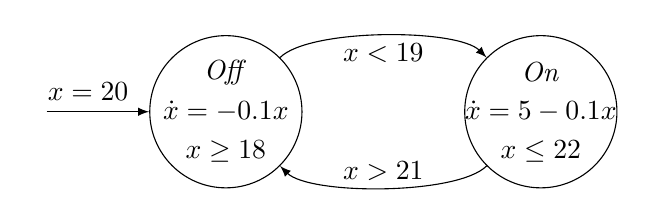
\begin{tikzpicture}[>=latex]
   
  \begin{scope}

%   \draw  (1,1) rectangle (7,1.5);

%\filldraw[black] (0,0) circle (2pt) node[anchor=west] {s};

  \node[circle, inner sep=2pt,draw, minimum height=55pt] (p1) at (-4,0) {};
      \node (p0_d) at (-4.0,0.5) {\textit{Off}};
      \node (p0_d) at (-4.0,0) {$\dot{x}=-0.1x$};
      \node (p0_d) at (-4.0,-0.5) {$x \geq 18$};
  
  \node[circle, inner sep=2pt,draw, minimum height=55pt] (p2) at (0,0) {};
      \node (p0_d) at (0.0,0.5) {\textit{On}};
      \node (p0_d) at (0.0,0) {$\dot{x}=5-0.1x$};
      \node (p0_d) at (0.0,-0.5) {$x \leq 22$};
  
     \draw[->] (p1) .. controls +(45:1.5) and +(135:1.5) .. (p2);
     \node (p0_d) at (-2.0,-0.75) {$x > 21$};
     
      \draw[->] (p2) .. controls +(-135:1.5) and +(-45:1.5) .. (p1);
      \node (p0_d) at (-2.0,0.75) {$x < 19$};
      
      
      \node (p0t) at (-5.75,0.25) {$x=20$};
      \node (p0) at (-6.40,-0.0) {};
        \draw[->] (p0) edge (p1);  
      
%       \draw[->] (p2) edge [loop right] node {} (p2);  
     
%     \node[circle, inner sep=2pt,draw, minimum height=20pt](p3) at (0.25,3) {on}; 
%     \node[circle, inner sep=2pt,draw, minimum height=20pt](p4) at (-0.5,1.5) {$\text{int}_2$}; 
%     
%     \node (p0_d) at (1.2,0) {$\inv:\dot T=0$};

  
%   \node (p0_d) at (1,1.8) {pre$_{\vdash}\cup$ pre$_{\vdash}^{\num}$};
%   \node (p1_d) at (4,1.8) {pre$_{\leftrightarrow}\cup$ pre$_{\leftrightarrow}^{\num}$};
%   \node (p2_d) at (7,1.8) {pre$_{\dashv}\cup$ pre$_{\dashv}^{\num}$};
% 
%   \node (p3_d) at (1.2,0.7) {eff$_{\vdash}^+\cup$ eff$_{\vdash}^-\cup$ eff$_{\vdash}^{\num}$};
%   \node (p5_d) at (4,0.7) {eff$_{\leftrightarrow}^{\num}$};
%   \node (p6_d) at (6.8,0.7) {eff$_{\dashv}^+\cup$ eff$_{\dashv}^-\cup$ eff$_{\dashv}^{\num}$};
% 
%     \node (p7_d) at (4,1.25) {$A$};
%   
  \end{scope}
\end{tikzpicture}
\caption{Thermostat hybrid automaton}
\label{fig:thermostat}
\end{figure*}

\subsection{PDDL2.1 and PDDL+ Planning}

Application of planners in real world problems has challenged the limitations of PDDL and increased the necessity of dealing with time and resources. This lead to the development of PDDL2.1~\cite{fox03} as the extension of PDDL able to model temporal domains. PDDL2.1 has been extended to PDDL+~\cite{pddl+} to enable the modelling of mixed discrete-continuous domains. In this section we first discuss the semantics of PDDL2.1 and later describe the extensions that have been added in PDDL+.

\begin{definition}[PDDL2.1 Planning]\label{def:pddl21}
A PDDL2.1 planning problem is a tuple $\Pi:=\{P,V,A,I,G\}$, where $P$ is a set of propositions; $V$ is a vector of real variables, called fluents; both are manipulated by $A$, a set of durative and instantaneous actions.
$I(P,V)$ is a function over $P\cup V$ which describes the \textit{initial state} of the problem and $G(P,V)$ is a function that describes the \textit{goal condition}.
\end{definition}

A durative action $a \in A$ is described as a tuple:
$$
a:=\{pre_{a},\mathit{eff}_{a},dur_{a}\}
$$
where $pre_{a}(P,V)$ is a function over $P\cup V$ that represents the action's preconditions -- conditions that must hold for the action to be applied. Similarly, $\mathit{eff}_{a}$ represents the action's effects, and $dur_{a}$ is a duration constraint, a conjunction of numeric constraints corresponding to the duration of the action $a$.

A single condition is either a single proposition $p\in P$, its negation, or a numeric constraint over $V$. A precondition is a conjunction of zero or more single conditions. The precondition of an action $pre_a$ can be separated into three disjoint subsets:
$$
pre_{\vdash a}, pre_{\leftrightarrow a}, pre_{\dashv a}\subseteq pre_{a}
$$
These represent the conditions that must hold at the start of the action, throughout its execution, and at the end of the action, respectively.

Action effects are described by seven subsets:
$$
\begin{array}{l}
\mathit{eff}^{+}_{\vdash a},\,\mathit{eff}^{-}_{\vdash a},\,\mathit{eff}^{num}_{\vdash a}, \\
\mathit{eff}^{+}_{\dashv a},\,\mathit{eff}^{-}_{\dashv a},\,\mathit{eff}^{num}_{\dashv a}, \\
\mathit{eff}_{\leftrightarrow a}
\end{array}
$$
The first six are the instantaneous effect of adding or removing propositions, or instantaneous numeric effects. These are bound to the start or end of the action. For example, $\mathit{eff}^{+}_{\vdash a}$ denotes the propositions added at the start of the action. In the semantics of PDDL2.1, the values of such instantaneous effects can be exploited to support other actions only after a small amount of time $\epsilon$~\cite{fox03}. This is referred to as \textit{epsilon separation}. The final set, $\mathit{eff}_{\leftrightarrow a}$ is a conjunction of \textit{continuous} numeric effects $\mathit{eff}_{\leftrightarrow}$, which are applied continuously while the action is executing. As a special case, \textit{instantaneous} actions have duration $0$, have only one set of preconditions $pre_a$; and three sets of effects $\mathit{eff}^{+}_a$, $\mathit{eff}^{-}_a$, and $\mathit{eff}^{num}_a$.

Actions can only be applied together at the same time if they are not mutually exclusive (mutex). Actions $a1$ and $a2$ can be applied simultaneously if:
$$
\begin{array}{c}
pre_{a1} \cap (\mathit{eff}^{+}_{a2} \cup \mathit{eff}^{-}_{a2} \cup \mathit{eff}^{num}_{a2}) = \emptyset \\
\mathit{eff}^{+}_{a1} \cap \mathit{eff}^{-}_{a2} = \mathit{eff}^{+}_{a2} \cap \mathit{eff}^{-}_{a1} = \emptyset \\
\{v1 \in \mathit{eff}^{num}_{a1}\} \cap \{v2 \in \mathit{eff}^{num}_{a2}\} = \emptyset \\
\end{array}
$$

PDDL+ is an extension of PDDL2.1, based on hybrid automata semantics. PDDL+ extends PDDL2.1 to support the modelling of exogenous events, reflecting changes that are initiated by the environment. These are introduced by the new constructs of \textit{processes} and \textit{events}.

\begin{definition}[PDDL+ Planning]\label{def:pddl+}
A PDDL+ planning problem is a tuple $\Pi+:=\big \langle P,V,A,Ps,E,I,G\big \rangle $, in which $P$ is a set of propositions; $V$ is a vector of real variables, called fluents; and $A$ is a set of durative and instantaneous actions. $Ps$ is a set of processes, and $E$ a set of events. $I(P,V)$ and $G(P,V)$ represent the initial state and goal condition respectively.
\end{definition}

The elements $P,V,A,I$, and $G$ are as in Definition~\ref{def:pddl21}. As an analogue, an event $e\in E$ is akin to an instantaneous action: if an event's preconditions $pre_e$ are satisfied, it occurs, yielding the event's instantaneous effects. Similarly, processes are akin to durative actions which apply continuous effects over a period of time.

Note that continuous processes are triggered as soon as their precondition becomes true, and in this sense they \textit{must} be triggered. Exogenous events follow the same semantics. The rationale behind this is that processes and events are used to model changes that are initiated by changes in the world, therefore they are not under the direct control of the executive and are triggered immediately (see Bogomolov et al.~\cite{bogomolov14} for more details). This is a critical distinction between processes/events and actions. The process/event will automatically occur as soon as its precondition is satisfied; whereas an action will only happen if chosen to be executed by the planner.

Furthermore, effects become instantaneously available to events, without the epsilon separation. This means, if one event $e1$ is triggered, with effects that satisfy another event $e2$ and trigger a process $p1$, then $e1$, $e2$, and the start of $p1$ all happen at exactly the same time-point. It is due to this behaviour that PDDL+ semantics place a bound on the number of cascading (parallel) events. According to PDDL+ semantics, a causal chain of events cannot include a cycle, and a single event cannot be triggered more than once in a single instant~\cite{fox2002pddl+}.

Given the PDDL+ semantics for modelling hybrid systems, finding an efficient planner that can handle events and processes is the next crucial step. A number of methods have been proposed to handle mixed discrete and continuous domains. We review these in Section~\ref{sec:related_work}.

\subsection{Planning as Satisfiability}

The problem of determining Boolean Satisfiability Problem (SAT) is the problem of finding an assignment of truth values to variables in order to make a set of propositional formulae true. The problem is stated as: given a Boolean expression $\phi$ with variables $X: \{ x_1, x_2, ... , x_n\}$, there exists an assignment to variables $X$ such that $\phi$ is satisfied? In other words:
$$
\exists \, x_1, x_2, ... , x_n \quad\phi?
$$
For example,
$$
\phi := (\neg x_1 \vee \neg x_2) \wedge (x_1 \vee x_3) \wedge (x_3 \vee x_2) \wedge \neg x_3
$$
is false, since there are no assignments to the three variables $x_1, x_2, x_3$ that will satisfy $\phi$.
%
In the context of planning, we are focusing on SAT solvers that solve the decision problem and if the expression is satisfiable, return an example satisfying assignment. Kautz and Selman~\cite{kau92} formalised propositional planning as a Boolean Satisfiability (SAT) problem in the following way.

First, the classical planning problem for a fixed horizon $n$ is modelled by defining $n$ copies of the Boolean variables which describe the state and actions, and unrolling $n$ times the transition relation that holds between states. This gives a set of variables ($X$) and constraints between them ($\phi$). A satisfying assignment to the variables corresponds to a plan trace.

In more detail, the set of variables $X$ comprises one Boolean variable for each $a\in A$, and each $p\in P$ \footnote{Similar to Definition~\ref{def:pddl21}, in classical planning we have a set of actions and a set of propositions which are shown as $A$ and $P$, respectively.} at each time-step $t_0, \ldots, t_n$. In propositional planning, there are no numeric variables $v\in V$. Constraints are added to $\phi$, asserting:
\begin{itemize}
\item The initial state holds at time-step $0$, and goals at time-step $n$.
\item If an action is true, then its preconditions hold in that time-step.
\item If an action is true, then its effects hold in the following time-step.
\item Two actions that are mutex cannot be applied together in the same time-step.
\end{itemize}

To solve the original planning problem without a fixed time horizon, an initial encoding with horizon $n_0$ is solved, and if found, the satisfying assignment is converted into a corresponding plan. Otherwise, the horizon is incremented and the process is repeated~\cite{kau99}.

A significant number of works have been devoted to formalising planning problems using propositional logic, and improving those encodings~\cite{rin06,che07,rob09,rin10,cas12b}, which we discuss in Section~\ref{sec:related_work}.

\subsection{Satisfiability Modulo Theory}

Satisfiability Modulo Theory (SMT)~\cite{bar18} is the problem of deciding the satisfiability of a first-order formula expressed in a given theory. An SMT problem is given as a set of variables and a set of constraints over those variables. In contrast to the SAT problem, the variables are not restricted to Boolean values, but depend upon a \textit{theory}, and the constraints are expressed with respect to a background \textit{logic}.
%
The theory and logic are critical elements of an SMT problem. Theories exist for Boolean propositions, finite and infinite trees, lists, bitvectors, arrays, integers, and reals. SMT takes advantage of the fact that some of them already have efficient solvers in order to reason more efficiently. In our work we use the theory of real numbers and the logic of \textit{quantifier-free non-linear real arithmetic}.

For example, an SMT problem in \textit{quantifier-free linear real arithmetic} might be:

$$
\exists u,v,x,y,z\quad\phi?
$$
where
$$
\phi:= (x+3 <= 2u) \vee (v+4 >= y) \vee (x+y+z >= 2)
$$

Problems in SMT can be expressed in the SMT-LIB standard syntax~\cite{bar10}. Figure~\ref{fig:smtlib} illustrates the example problem above in the standard sytax. The encoding we describe in this paper is produced in this standard format, and can be read many SMT solvers, including {\sc z3}~\cite{dem08}, which we use to solve our problems in Section~\ref{sec:experiments}. 

\begin{figure}[htb]
\centering
\begin{BVerbatim}
( set-logic QF_LRA )
( declare-fun u () Real)
( declare-fun v () Real)
( declare-fun x () Real)
( declare-fun y () Real)
( declare-fun z () Real)
( assert
    (or
    ( <= (+ x 3) (* 2 u ) )
    ( >= (+ v 4) y )
    ( >= (+ x y z ) 2)
    )
)
\end{BVerbatim}
\caption{SMT problem in the SMT-LIB standard syntax.}
\label{fig:smtlib}
\end{figure}

\section{Working Example}\label{sec:working_example}

For the purpose of clarity and ease, we have chosen a simple \emph{Free Fall} problem as our working example and we use this problem to indicate different concepts explained throughout this paper. 

In the first part of this section we explain the \emph{Free Fall} problem, and later we describe the hybrid automaton corresponding to this problem. Finally, we provide the PDDL+  model of our problem and map the hybrid automaton to the PDDL+ model. We will then present the SMT encoding of this problem in Section~\ref{sssec:Free_Fall}.

\subsection{Free Fall Problem}

%\begin{definition}[Free Fall Problem]
%\emph{Free Fall} is any motion of a body where gravity is the only force acting upon it.
%\end{definition}
%$\qed$	

Our working example considers a ball that falls vertically under the influence of gravity ($g$) and bounces when it touches the floor. The goal is for a robotic hand to catch the ball. Specific conditions will be defined for the robot which determine when to catch the ball (i.e. at a specific time or position, or after a specific number of bounces), as shown in Figure~\ref{fig:Freefall}. It is important to note that Figure~\ref{fig:Freefall} shows the real case of a bouncing ball, however in our working example the motion is idealised as other forces and their effects (i.e. air resistance) are assumed to be negligible (so the ball will bounce an infinite number of times and every time reach to its initial height). The ball can be released with an initial velocity of zero ($v_0 = 0$) or it can have an initial velocity of $v_0$.

\begin{figure}[!ht]
\centering
\includegraphics[width=0.60\textwidth]{diagrams/FreeFall2.png}
\caption{Working example (Free Fall problem): indicates a ball that is released vertically from the initial height of $h_0$ and bounces as soon as it reaches the floor. The diagram shows two different goal conditions we can specify for the robot to catch the ball; at a specific height ($h_{goal}$) or at a specific time after releasing the ball ($t_{caught}$).}
\label{fig:Freefall}
\end{figure}

% Also it is important to define a positive direction for the height, velocity and acceleration. As you can see in Figure~\ref{fig:Direction_Freefall}, in this problem any vector that is directed downwards is positive. By this mean the velocity $v$ has a positive values when the ball is falling and it become negative as soon as the ball bounces and the direction of movement becomes upward. However, acceleration and height has always positive values.

% In the next part, in order to show the discrete and continuous nature of the changes in our working problem, we develop the hybrid automaton this problem.

% \begin{figure}[!ht]
% \centering
% \includegraphics[width=0.350\textwidth]{diagrams/Direction_Freefall.png}
% \caption{In our working example (Free Fall problem) we chose a positive direction for velocity, height and the acceleration}
% \label{fig:Direction_Freefall}
% \end{figure}

\subsection{Hybrid Automaton: Free Fall Problem}

The hybrid automaton of the Free Fall problem is shown in Figure~\ref{fig:Free Fall hybrid automaton}. In this problem the height and velocity of the ball are represented by the continuous variables $h$ and $v$, respectively. The acceleration of the ball due to gravity is represented by the variable $a$.

% DROPPING BALL HYBRID AUTOMATON
\begin{figure*}[ht]
\centering
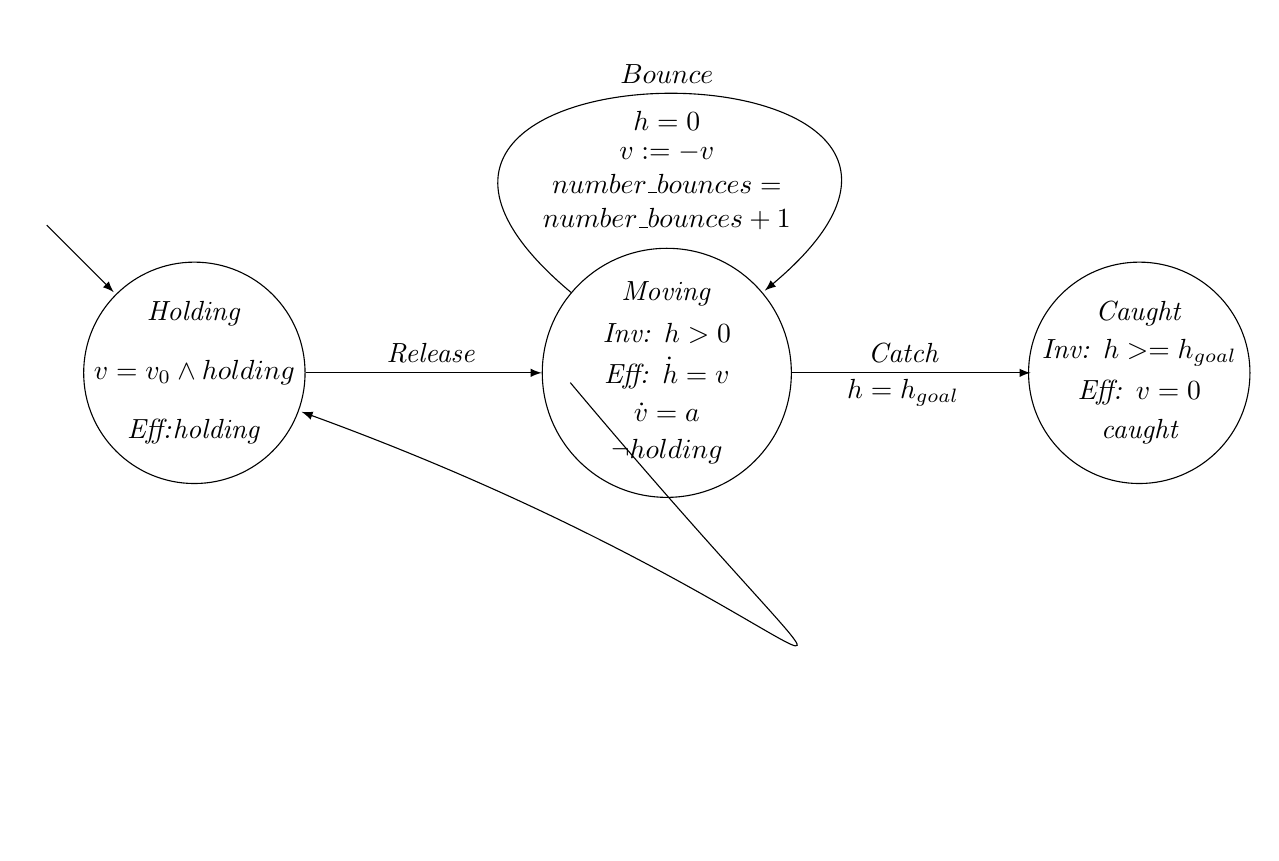
\begin{tikzpicture}[>=latex]
  \begin{scope}

%   \draw  (1,1) rectangle (7,1.5);

%\filldraw[black] (0,0) circle (2pt) node[anchor=west] {s};
\node (p1) at (-6,0.0) {};
\node (p2) at (-1.33,0.0) {};
\node (p3) at (4.745,0.0) {};




\node[circle, inner sep=4pt,draw, minimum height=80pt] (p1) at (-6,0) {};
\node (p4) at (-8,2.0) {};

\draw[->,shorten >=1pt] (p4) to  (p1);
\node (p0_d) at (-6.0,0.75) {\textit{Holding}};
%\node (p0_d) at (-6.0,0.25) {\textit{Inv:}   $h=h_0$};
\node (p0_d) at (-6.0,0){$v=v_0 \wedge holding $};
\node (p0_d) at (-6.0,-0.75) {\textit{Eff:}\textit{holding}};
\node (p0_d) at (-3.0,0.25) {$\textit{Release}$};
\draw[->,shorten >=1pt] (p2) to [out=310,in=340,loop,looseness=5.5] (p1);
\node (p0_d) at (-3.0,-0.25) {};

\node[circle, inner sep=4pt,draw, minimum height=90pt] (p2) at (0,0) {};
\draw[->] (p1) edge (p2);

\node (p1_d) at (0.0,1.0) {\textit{Moving}};
\node (p1_d) at (0.0,0.5) {\textit{Inv:} $h>0$};
\node (p1_d) at (0.0,0.0) {\textit{Eff:}  $\dot{h}=v$};
\node (p1_d) at (0.0,-0.5) {$\dot{v}=a$};
\node (p1_d) at (0.0,-1.0) {$\neg holding$};
\draw[->] (p2) edge (p3);
\node (p1_d) at (3.0,0.25) {$\textit{Catch}$};
\node (p1_d) at (3.0,-0.25) {$h=h_{goal}$};
\draw[->,shorten >=1pt] (p2) to [out=140,in=40,loop,looseness=5.5] (p2);
\node (p1_d) at (0.0, 3.2) {$h=0$};
\node (p1_d) at (0.0, 2.8) {$v:=-v$};
\node (p1_d) at (0.0, 2.4) {$number\_bounces = $};
\node (p1_d) at (0.0, 1.95) {$number\_bounces + 1 $};
\node (p1_d) at (0.0, 3.8) {$Bounce$};

\node[circle, inner sep=4pt,draw, minimum height=80pt] (p3) at (6,0) {};
\node (p2_d) at (6.0,0.75) {\textit{Caught}};
\node (p2_d) at (6.0,0.25) {\textit{Inv:}   $h>=h_{goal}$};
\node (p2_d) at (6.0,-0.25){\textit{Eff:}  $v=0$};
\node (p2_d) at (6.0,-0.75) {$\textit{caught}$};
\end{scope}
\end{tikzpicture}
\caption{Free Fall hybrid automaton}
\label{fig:Free Fall hybrid automaton}
\end{figure*}

Considering the dynamics of the problem, we have three discrete locations. The initial state which indicates our first discrete mode: the ball is held at the height $h_0$ and the velocity $v = v_0$ (this state is shown by the left circle in Figure~\ref{fig:Free Fall hybrid automaton}). As soon as the ball is released, a discrete transition moves the automaton to the next discrete location representing the moving state (this state is shown by the middle circle in Figure~\ref{fig:Free Fall hybrid automaton}). In this state, the height of the ball changes according to the velocity $\dot{h}=v$, and the velocity changes according to acceleration $\dot{v}=a$. As soon as the height of the ball becomes zero ($h=0$), the ball bounces. A discrete transition negates the velocity.

The robot can catch the ball as soon as the conditions of the goal state are satisfied. In Figure~\ref{fig:Free Fall hybrid automaton} this condition is that the ball is at a specific height $h=h_{goal}$. At this point, the hybrid automaton will move to the next discrete state which represents the state where the ball has been caught by the robot (this state is shown by the right circle in Figure~\ref{fig:Free Fall hybrid automaton}).

\subsection{PDDL+ Model of the Free Fall Problem}

In this section we describe how the hybrid automaton of the Free Fall problem can be written in PDDL+. A planning model represented in PDDL+ consists of the domain and the problem instance. The domain model lists the action schema and the possible processes and events. The problem instance describes the objects, the initial state, and the goal state. The domain corresponding to the hybrid automaton in Figure~\ref{fig:Free Fall hybrid automaton} is shown in Figure~\ref{fig:freefall domain}, while the problem instance is shown in Figure~\ref{fig:freefall problem}. In this problem we include a single ball, \textit{ball1}, and define that the robot should catch the ball when the height of the ball is 5.

\begin{figure*}[thb]
\small
\begin{BVerbatim}
(define (domain dropping_ball)
(:requirements :fluents :typing :durative-actions :time :negative-preconditions :duration-inequalities :timed-initial-literals) ;;:durative-actions :time :negative-preconditions :duration-inequalities

(:types ball)
(:predicates (holding ?b - ball) (caught ?b - ball))
(:functions
    (velocity ?b - ball)
    (height ?b - ball)
    (catch_height)
    (number_bounces ?b - ball)
    (catch_bounce)
)

(:action release
 :parameters (?b - ball)
 :precondition (and (holding ?b) (= (velocity ?b) 0))
 :effect (and (not (holding ?b)))
)

(:process moving
 :parameters (?b - ball)
 :precondition (and (not (holding ?b)) (>= (height ?b) 0))
 :effect (and
    (increase (velocity ?b) (* #t -9.8) )
    (increase (height ?b) (* #t (velocity ?b))))
 )
 
(:event bounce
 :parameters (?b - ball)
 :precondition (and (< (velocity ?b) 0) (<= (height ?b) 0.000001))
 :effect (and 
    (increase (number_bounces ?b) 1)
    (assign (velocity ?b) (* -1 (velocity ?b))))
)

(:action catch
 :parameters (?b - ball)
 :precondition (and
    (>= (height ?b) (catch_height))
    (<= (height ?b) (+ (catch_height) 0.1))
    (>= (number_bounces ?b) (catch_bounce)))
 :effect (and
    (holding ?b)
    (assign (velocity ?b) 0)
    (caught ?b)))
)

\end{BVerbatim}
\caption{Simplified PDDL+ domain description for Free Fall.}
\label{fig:freefall domain}
\end{figure*}

% working example problem (Free fall)
\begin{figure*}[thb]
\small
\centering
\begin{BVerbatim}
(define (problem dropping_ball_1)
(:domain dropping_ball)
(:objects ball1 - ball)

(:init 
    (holding ball1)
    (= (velocity ball1) 0)
    (= (height ball1) 10)
    (= (catch_height) 5)
    (= (number_bounces ball1) 0)
    (= (catch_bounce) 1)
)

(:goal
    (caught ball1)
))
\end{BVerbatim}
\caption{Simplified PDDL+ Free Fall problem file}
\label{fig:freefall problem}
\end{figure*}

Grounding the problem by applying the objects from the problem instance to the predicates of the domain forms the propositional variables $(holding\ ball1)$ and $(caught\ ball1)$. These variables describe a discrete state-space of 4 states:
\begin{itemize}
\item The initial state in which $(holding\ ball1)$ is true and $(caught\ ball1)$ corresponds to the \emph{Holding} location of the hybrid automaton.
\item The state in which both variables are false is reached after applying the action $(release\ ball1)$. This state corresponds to the \emph{Moving} location of the hybrid automaton. In this discrete state, the process $(moving\ ball1)$ asserts the continuous change on the numeric variables.
\item The state where both variables are true, is reached by applying the action $(catch\ ball1)$. This state corresponds to the \emph{Caught} location in the hybrid automaton. The goal holds in this state.
\item The state in which $(holding\ ball1)$ is false and $(caught\ ball1)$ is true is not reachable from the initial state without first reaching the goal, and does not appear in the hybrid automaton.
\end{itemize}

The continuous change of the location \emph{Moving} is asserted by the process $(moving\ ball1)$, which is active while its preconditions, $(not (holding\ ball1))$ and $(>= (height\ ball1)\ 0)$, are satisfied. The event $(bounce\ ball1)$ has no effect upon the discrete state, instead affecting only the numeric variables and also increases the $(number\_bounces)$. This event corresponds to the self-looping transition \emph{Bounce} in the hybrid automaton. As explained previously, an event is triggered as soon as its preconditions are satisfied. In this case, the event will be triggered as soon as the ball has reached the floor. This precondition is shown as $(<= \ (height \  ?b) \ 0.000001)$. Note that in the automaton, the transition \emph{Bounce} is a must transition, in the sense that is a must be triggered as soon as $h=0$ as this violates the invariant of \emph{Moving}. Similarly, events in PDDL+ follow a must semantics and are triggered as soon as their preconditions are satisfied. 
%The reason for modelling this precondition as an inequality less than or equal to a small constant is to get a valid plan using the validator~\cite{howey2004val}.

\section{Encoding PDDL+ Domains in SMT}\label{sec:enc}

In this section we describe how we encode a PDDL+ domain into SMT. First we describe the basic elements of the encoding, the happening and later we expand the encoding for the whole planning problem.

\subsection{Encoding of a single happening}\label{sec:enc_happening}

Our encoding is based on the notion of \textit{happening}, which is used to capture the discrete change in the state at a given time point due to the effects of actions, processes, or events. Namely, each happening encodes the causal chain of events, processes and instantaneous actions which might occur simultaneously at a given time point. We have defined a bound $B$ as the length of the causal cascading instantaneous events and we split durative actions as two instantaneous actions, representing the start and end of the action, and one process representing the continuous numeric effects and invariant.

\begin{definition}[Happening]
A happening is the tuple $x := \{P, V, E, Ps, A \}$, where:
\begin{itemize}

\item ${P}=\{P_{0},\ldots,P_{B+1}\}$ are the propositional state variables at happening $x$, in $B+1$ layers;

\item ${V}=\{V_{0},\ldots, V_{B+1}\}$ are the real state variables at happening $x$, also in $B+1$ layers;

\item ${E}=\{E_{0},\ldots,E_{B}\}$ represents the chain of events triggered at happening $x$. The chain is of length $B$;

\item ${Ps}$ represents the set of processes active over the next interval;

\item ${A}$ is the set of actions applied at the happening.
\end{itemize}
\label{def:happening}
\end{definition}
 
Each $P_{i}$ is a set of all the propositions, i.e.:
$$
P_{i} = \{p_{i}, \forall p \in P\} , i\in \{0,\ldots, B+1\}
$$

Similarly we have the following for the $V_{i}$ and $E_{i}$:
$$
\begin{array}{cc}
V_{i} = \{v_{i}, \forall v \in V\}, & i\in \{0,\ldots, B+1\}\\
E_{i} = \{e_{i}, \forall e \in E\}, & i\in \{0,\ldots, B\}
\end{array}
$$

An example of happening is shown in Figure~\ref{fig:happening}. The chain of events forms a set of layers at each happening. Each circle in Figure~\ref{fig:happening} represents a layer. The number of event steps in each happening is bounded to $B$. The last layer indicates the final value of the state variables after considering the effects of the cascading events. If the causal chain of events is longer than this bound, then a valid plan will not be found.

\begin{figure}[ht]
\centering


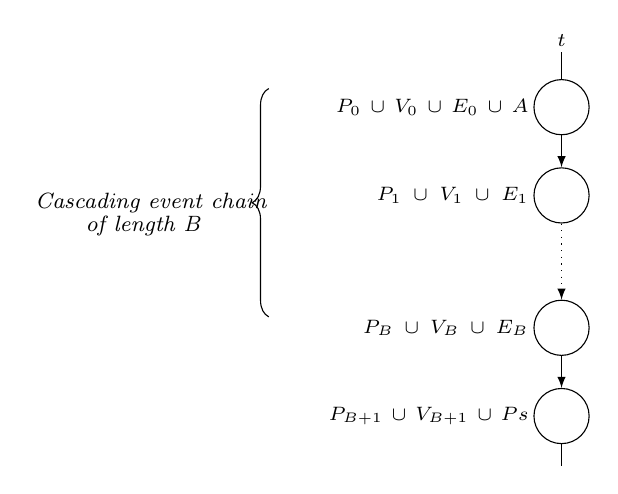
\begin{tikzpicture}[>=latex]
  \begin{scriptsize}
  \begin{scope}

  \node[align=center] (t1) at (0em,3em) {$t$};

  
  \draw (0em,2.5em) -- (0,1.25em);
 

  \node[circle, inner sep=0em, draw, minimum size=2.5em] (b0) at (0em,0) {};
  \node[align=right, text width=12em] (b0e) at (-7.5em,0) {$P_{0}\cup V_{0}\cup E_{0}\cup A$};

  \node[circle, inner sep=0em, draw, minimum size=2.5em] (b1) at (0em,-4em) {};
  \node[align=right, text width=12em] (b1e) at (-7.5em,-4em) {$P_{1}\cup V_{1}\cup E_{1}$};

  \node[circle, inner sep=0em, draw, minimum size=2.5em] (b2) at (0em,-10em) {};
  \node[align=right, text width=12em] (b2e) at (-7.5em,-10em) {$P_{B}\cup V_{B}\cup E_{B}$};
 
 \node[circle, inner sep=0em, draw, minimum size=2.5em] (bb) at (0em,-14em) {};
 
 \node[align=right, text width=12em] (bbe) at (-7.5em,-14em) {$P_{B+1}\cup V_{B+1}\cup Ps$};

  
  \draw (0em,-15.25em) -- (0,-16.25em);


  \draw[->] (b0) -- (b1);
  \draw[->, dotted] (b1) -- (b2);
  \draw[->] (b2) -- (bb);
  
  
\draw [decorate,decoration={brace,amplitude=6pt},xshift=-120pt,yshift=-90pt]
(0.5,0.5) -- (0.5,3.4) node [black,midway,xshift=-1.5cm] 
{\footnotesize $\textit{Cascading event chain}$} node [black,midway,xshift=-1.6cm, yshift=-0.3cm] 
{\footnotesize $\textit{of length B}$};

  \end{scope}
  \end{scriptsize}
\end{tikzpicture}

\caption{A single happening occurs at time $t$, and includes several sets of state variables. These sets describe a causal chain of instantaneous events.}
\label{fig:happening}
\end{figure}

Following from Definition~\ref{def:happening}, happening $x_t$ is encoded by the SMT variables:
$$
x_t:=\Bigg \langle 
\begin{array}{l}
\qquad time_t,\\
\qquad P_{0,t},\ldots,\,P_{B+1,t},\\
\qquad V_{0,t},\ldots,\,V_{B+1,t},\\
\qquad E_{0,t},\ldots,\,E_{B,t},\\
\qquad Ps_t,\,A_t,\,\\
\qquad flow_{V_t},\,dur_{Ps_t}
\end{array}
\Bigg \rangle 
$$

The happenings in our encoding either describe a moment of discrete change -  which corresponds to the discrete transition \textit{Trans} of the hybrid automata - or a point in time between moments of discrete change in which the derivative is equal to zero for some numeric continuous change. The latter case is to ensure that invariant conditions hold, avoiding the case described later in Figure~\ref{fig:Zero_cross}. Between happenings there is only continuous numeric change (\textit{Flow}). The key difference between a hybrid automaton and the SMT encoding is that multiple actions can be performed in a single happening in parallel, meaning that while the hybrid automaton is exponential in the size of the PDDL+ description, our encoding will be linear.

The set $flow_{V_{t}}:=\{flow_{{v_t}} | \forall v_t\in V_t\}$ is a set of numeric expressions that represent the change in value of each numeric variable $v$ from this time point to the next. The variables $dur_{{Ps_t}}:=\{dur_{ps_t} | \forall ps_t\in Ps_t\}$ represents the remaining duration of each process. $dur_{ps}$ and is constrained to be positive if and only if the process is currently executing.

The constraints within a happening are shown in Figure~\ref{eq:state}. 

\begin{figure*}[thb!]
% \begin{minipage}[t]{0.58\linewidth}
\textbf{Proposition and real variable support}
\begin{enumerate}[label=H\arabic*.]
 % Literal support
  \item $\bigwedge_{p \in P} p_{1,t} \rightarrow (p_{0,t} \vee \bigvee_{e \in E | p \in eff^{+}_{e}} e_{0,t} \vee \bigvee_{a_t \in A | p \in eff^{+}_{a}} a_t)$
  \item $\bigwedge_{p \in P} \neg p_{1,t} \rightarrow (\neg p_{0,t} \vee \bigvee_{e \in E | p \in eff^{-}_{e}} e_{0,t} \vee \bigvee_{a \in A | p \in eff^{-}_{a}} a_t)$
  \item $\bigwedge_{i=1}^{B} \bigwedge_{p \in P} p_{i+1,t}      \rightarrow (     p_{i,t} \vee \bigvee_{e \in E | p \in eff^{+}_{e}} e_{i,t})$
  \item $\bigwedge_{i=1}^{B} \bigwedge_{p \in P} \neg p_{i+1,t} \rightarrow (\neg p_{i,t} \vee \bigvee_{e \in E | p \in eff^{-}_{e}} e_{i,t})$
 % Real variable support
  \item $\bigwedge_{v \in V} (\bigwedge_{a \in A | v \in eff^{num}_{a}} \neg a_{t} \wedge \bigwedge_{e \in E | v \in eff^{num}_{e}} \neg e_{0,t}) \rightarrow (v_{i+1,t} = v_{i,t})$
  \item $\bigwedge_{i=1}^{B} \bigwedge_{v \in V} (\bigwedge_{e \in E | v \in eff^{num}_{e}} \neg e_{i,t}) \rightarrow (v_{i+1,t} = v_{i,t})$
\end{enumerate}
\textbf{Event preconditions and effects}
\begin{enumerate}[label=H\arabic*.]\setcounter{enumi}{6}
 % event preconditions
 \item $\bigwedge_{i=0}^{B} \bigwedge_{e \in E} e_{i,t} \leftrightarrow pre_{e} (P_{i,t} \cup V_{i,t})$
 % event effects
 \item $\bigwedge_{i=0}^{B} \bigwedge_{e \in E} e_{i,t} \rightarrow eff_{e} (P_{i+1,t} \cup V_{i+1,t})$
\end{enumerate}
% \end{minipage}
% \begin{minipage}[t]{0.42\linewidth}
\textbf{Action preconditions and effects}
\begin{enumerate}[label=H\arabic*.]\setcounter{enumi}{8}
 % Action preconditions
 \item $\bigwedge_{a \in A} a_t \rightarrow pre_{a}(P_{0,t} \cup V_{0,t})$
  % action effects
 \item $\bigwedge_{a \in A} a_t \rightarrow eff_{a}(P_{1,t} \cup V_{1,t})$
\end{enumerate}
\textbf{Process triggering}
\begin{enumerate}[label=H\arabic*.]\setcounter{enumi}{10}
 % process triggering
 \item $\bigwedge_{ps\in Ps} ps_t \leftrightarrow pre_{ps}(P_{B+1,t} \cup V_{B+1,t})$
 \item $\bigwedge_{ps\in Ps} dur_{ps_t} >= 0$
 \item $\bigwedge_{ps\in Ps} ps_t \leftrightarrow (dur_{ps_t} > 0)$
\end{enumerate}
\textbf{Action mutexes}
\begin{enumerate}[label=H\arabic*.]\setcounter{enumi}{13}
 % Action mutexes
 \item $\bigwedge_{a \in A} \bigwedge_{a' \in A | a \nparallel a'} (\neg a_t \vee \neg a'_t)$
\end{enumerate}
% \end{minipage}
\caption{Encoding of a PDDL+ happening to SMT.}
\label{eq:state}
\end{figure*}

\smallskip

\begin{itemize}

\item Proposition and real variable support

These constraints ensure that the value of propositions (H1-H4) and real variables (H5-H6) remains consistent from $P_{0,t}\cup V_{0,t}$ to $P_{B+1,t}\cup V_{B+1,t}$. Constraints (H1) and (H2) enforce the correct values after considering the add and delete effects of the initial events ($E_{0,t}$) and actions (${A_t}$). Similarly, constraints (H3) and (H4) enforce the propositional add and delete effects throughout the instantaneous chain of events. (H5) enforces the numeric effects of the initial events and actions. (H6) enforces the numeric effects of the remaining events. Note that after the first layer at each happening there are only events, and no actions.

\item Event preconditions and effects

This set of constraints enforces that an event is triggered if and only if its precondition holds (H7) and that if an event is triggered, its effects are present in the next layer of that happening (H8).

\item Action preconditions and effects

Similar to (H6-H7), these constraints ensure for actions $A_t$ that their preconditions must hold in $P_{0,t}\cup V_{0,t}$ (H9) and their effects are enforced in $P_{1,t}\cup V_{1,t}$ (H10).

\item Process triggering

This group of constraints enforce that a process is active if and only if its preconditions are satisfied in set $P_{B+1,t}\cup V_{B+1,t}$ (H11). It also enforces that the real variable $dur_{ps_t}$ for each process is greater than or equal to zero (H12), and strictly greater that zero if and only if the process is active at the end of the causal chain of events (H13). These constraints will be used to ensure that a process cannot finish outside of a happening.

\item Action mutexes

This set of binary constraints enforces that no two mutex actions can be applied simultaneously. For each pair of mutex actions, denoted $a_t \nparallel a'_t$, at least one must be false (H14).

\end{itemize}

\subsection{Encoding of a Plan}\label{sec:enc_problem}

Having defined happenings, a PDDL+ problem $\Pi+$ can be encoded as a bounded number of happenings $X:=\{x_1,\ldots,x_n\}$, such that any proof for the SMT formula represents the trace of a valid plan for $\Pi+$. The \textit{plan} corresponding to that trace is the set of action assignments $A_1\cup \ldots\cup A_n$.\footnote{As processes and events do not appear in a PDDL+ plan.}

Therefore, the existence of a plan for a  {\sl PDDL+ planning problem $\Pi+$ with bound $n$} is proved by building the SMT formula $\Pi+_n$ in the theory of quantifier-free (nonlinear) real arithmetic with $n$ copies of the set of happening variables $X = \{x_1,\ldots,x_n\}$ for $n \geq 1$. A \textit{plan for $\Pi+$} is the assignment to the action variables in any proof of $\Pi+_n$. The encoding is illustrated by Figure~\ref{fig:plan}.

\begin{figure*}[thb]
\center
\begin{tikzpicture}[>=latex]
  \begin{scriptsize}
  \begin{scope}

  % Initial and goal

  \node[align=right, text width=4em] (b0e) at (-6em,0) {\large $I$};
  \draw (-3em,0em) -- (2em,0em);
  \node[circle, inner sep=0em, draw, minimum size=0.5em, fill=black] at (2em,0em) {};
  
  \node[align=left, text width=4em] (b0e) at (50em,-5em) {\large $G$};
  \draw (42em,-5em) -- (47em,-5em);
  \node[circle, inner sep=0em, draw, minimum size=0.5em, fill=black] at (42em,-5em) {}; 
  
  % Happening 1
  
  \node[align=center] at (2em,4em) {\large $x_1$};
 
  
  \draw (2em,1.5em) -- (2em,1em);

  \node[circle, inner sep=0em, draw, minimum size=2.0em] (b01) at (2em,0) {};
  \node[circle, inner sep=0em, draw, minimum size=2.0em] (b11) at (2em,-2em) {};
  \node[circle, inner sep=0em, draw, minimum size=2.0em] (bb1) at (2em,-5em) {};


  \draw (2em,-6em) -- (2em,-8em);
  
  \draw[->, dotted] (b11) -- (bb1);
 
  
  % Happening 2

  \node[align=center] at (12em,4em) {\large $x_2$};
 
  
  \draw (12em,1.5em) -- (12em,1em);


  \node[circle, inner sep=0em, draw, minimum size=2.0em] (b02) at (12em,0) {};
  \node[circle, inner sep=0em, draw, minimum size=2.0em] (b12) at (12em,-2em) {};
  \node[circle, inner sep=0em, draw, minimum size=2.0em] (bb2) at (12em,-5em) {};


  \draw (12em,-6em) -- (12em,-8em);

  
  \draw[->, dotted] (b12) -- (bb2);
  
  
  % Happening 3
  
  \node[align=center] at (22em,4em) {\large $x_3$};
  
 
  \draw (22em,1.5em) -- (22em,1em);


  \node[circle, inner sep=0em, draw, minimum size=2.0em] (b03) at (22em,0) {};
  \node[circle, inner sep=0em, draw, minimum size=2.0em] (b13) at (22em,-2em) {};
  \node[circle, inner sep=0em, draw, minimum size=2.0em] (bb3) at (22em,-5em) {};


  \draw (22em,-6em) -- (22em,-8em);
 
  
  \draw[->, dotted] (b13) -- (bb3);
 

  % Happening 4
  
  \node[align=center] at (42em,4em) {\large $x_n$};
  
  \draw (42em,1.5em) -- (42em,1em);


  \node[circle, inner sep=0em, draw, minimum size=2.0em] (b04) at (42em,0) {};
  \node[circle, inner sep=0em, draw, minimum size=2.0em] (b14) at (42em,-2em) {};
  \node[circle, inner sep=0em, draw, minimum size=2.0em] (bb4) at (42em,-5em) {};
 

  \draw (42em,-6em) -- (42em,-8em);

  
  \draw[->, dotted] (b14) -- (bb4);

  
  
  % Inter-happening edges
  
  \draw (bb1) edge[out=0,in=180,->] (b02);
  \draw (bb2) edge[out=0,in=180,->] (b03);
  \draw[dotted] (26em,-4em) -- (37em,-4em);
  
  \end{scope}
  \end{scriptsize}
\end{tikzpicture}
\caption{A plan is found by building a formula with $n$ copies of the set of variables $x_t$ for $t = 1 \ldots n$. Each Happening models discrete change. Between happenings there is only continuous numeric change. The initial state is modelled in $t_1$, and the goal constraints are added to $t_n$.}
\label{fig:plan}
\end{figure*}

\noindent The constraints for a happening in Figure~\ref{eq:state} are copied for each happening $x_1 \ldots x_n$. Additional constraints in the SMT formula $\Pi+_n$ are shown in Figure~\ref{eq:plan} and explained below.

\begin{figure*}[thb]
\begin{minipage}[t]{0.39\linewidth}
\textbf{Instance description}
\begin{enumerate}[label=P\arabic*.]
  % Known states
  \item $I(P_{0,1}\cup V_{0,1})$
  \item $G(P_{B+1,n}\cup V_{B+1,n})$
  % Timing of happenings
  \item $time_0 = 0$
  \item $\bigwedge_{i=2}^n time_i \geq time_{i-1}+\epsilon$
\end{enumerate}
\textbf{Proposition support}
\begin{enumerate}[label=P\arabic*.]\setcounter{enumi}{4}
  % Literal support
  \item $\bigwedge_{i=2}^n \bigwedge_{p\in P} p_{0,i} \rightarrow p_{B+1,i-1}$
  \item $\bigwedge_{i=2}^n \bigwedge_{p\in P} \neg p_{0,i} \rightarrow \neg p_{B+1,i-1}$
\end{enumerate}
\end{minipage}
\begin{minipage}[t]{0.6\linewidth}
\textbf{Invariants}
\begin{enumerate}[label=P\arabic*.]\setcounter{enumi}{6}
  % Process timing conditions (these are necessary in combination to ensure happenings occur at dur=0)
  \item $\bigwedge_{i=2}^n \bigwedge_{ps\in Ps} ps_{i-1} \rightarrow dur_{ps_i} = dur_{ps_{i-1}} - time_i + time_{i-1}$
  % Interval constraints
  \item $\bigwedge_{i=1}^{n-1} \bigwedge_{ps \in Ps}  ps_i \leftrightarrow pre_{\leftrightarrow ps_i}$
  \item $\bigwedge_{i=1}^{n-1} \bigwedge_{e\in E} \neg pre_{\leftrightarrow e_i}$
\end{enumerate}
\textbf{Continuous change on real variables}
\begin{enumerate}[label=P\arabic*.]\setcounter{enumi}{9}
 % Vector flows
  \item $\bigwedge_{i=1}^{n-1} \bigwedge_{v\in V} flow_{v_i} = \int^{time_{i+1}}_{time_i} \sum_{ps\in Ps} eff^{num}_{\leftrightarrow ps}(V_i)dt$
  \item $\bigwedge_{i=2}^n \bigwedge_{v\in V} (v_{0,i} = v_{B+1,i-1} + flow_{v,i-1})$
\end{enumerate}
\end{minipage}
\caption{Encoding of PDDL+ planning problem $\Pi+$ to SMT.}
\label{eq:plan}
\end{figure*}

% According to the PDDL2.1 and PDDL+ epsilon separation semantics, effects can be exploited by actions $\epsilon$ time after they occur, therefore we need to apply the changes at time point $t+\epsilon$. Formally, we have the following 

\begin{itemize}

\item Instance description

These constraints enforce the initial state to hold in the first happening (P1), and that the goal is achieved in the final happening (P2). Following PDDL2.1 and PDDL+ semantics, they constrain the timing of happenings to enforce epsilon separation (P3-P4).

\item Proposition support

These constraints ensure that the discrete state variables do not change between happenings (P5-P6).

\item Invariants

These constraints ensure that the continuous numeric change between happenings does not violate any invariant constraints. First (P7) ensures that if a process is active in the previous happening, its duration is decreased by the time between happenings. This constraint, in combination with constraints (H12-H13) of Figure~\ref{eq:state}, ensure that a process cannot end between happenings. A process can remain active over intervals spanning multiple happenings.

Constraint (P8) enforces the invariant of the process. If a process is active, then the precondition of the process is active over the whole interval between happenings, and if the process is not active, then its preconditions are false over the whole interval. For constraints over real valued variables, this is done by checking the value either side of the interval. For nonlinear change, this is not sufficient (as shown in Figure~\ref{fig:Zero_cross}). It is necessary to include the following additional constraint:
$$
ps_{t_j} \rightarrow \bigwedge^{A_{t_j}}_{a_{t_j}=1} \left((\frac{d^af}{dt^a})_j(\frac{d^af}{dt^a})_{j+1} >= 0\right); 
$$
where $f$ is the numeric, non-constant part of the invariant, and where the $(A+1)$th derivative of $f$ is identically zero. This ensures that the derivatives of the function do not cross zero over the interval, thus a fluctuating value of $f$ cannot violate the invariant condition between $t_j$ and $t_{j+1}$.

\begin{figure*}[htb!]
\center

\usepgfplotslibrary{fillbetween}

\begin{tikzpicture}[domain=-2:2]

%\draw[->] (-3.5,0) -- (3.5,0)
%node[below right] {$x$};
%\draw[->] (0,-2) -- (0,3.5)
%node[left] {$y$};
%\draw plot[id=x] function{-(x*x)+3};
%\end{tikzpicture}


\begin{axis}[
    xmin=-4, xmax=4,
    ymin=-4, ymax=4
    ]

    \addplot [name path=plot1, ultra thin, domain=-10:10, samples=150]{-(x*x)+2}; 
    \addplot [name path=plot2, ultra thin, domain=-8:8]{1};
\addplot[thick, samples=50, smooth,domain=-4:4,magenta, name path=three] coordinates {(2,-4)(2,4)} ;
\addplot[thick, samples=50, smooth,domain=-4:4,magenta, name path=three] coordinates {(-2,-4)(-2,4)};

    

    \addplot[red] fill between[of=plot1 and plot2, soft clip={domain=-1:1}];
    

\end{axis}
\end{tikzpicture}
\caption{The plot illustrates continuous non-linear numeric change between two time points, indicated by vertical lines. While considering the non-linear change, we need to check whether the invariant condition of a process is satisfied throughout the interval. If the invariant asserts that the function should remain below the horizontal line, the figure shows that it is not sufficient to check the value of the function only at the time points.}
\label{fig:Zero_cross}
\end{figure*}

Constraint (P9) similarly ensures that an event is not triggered during an interval.

\item Continuous change on real variables

These constraints enforce continuous change over the interval (P10), applying the result to each real variable (P11). In order to calculate the change, the indefinite integral of the process' effects upon the variable must be computed. This is done automatically using the computer algebra systems (CAS) SymPy~\cite{sympy} and Piranha~\cite{bis18}.

For example, consider the process of the ball falling in the working example. The ball is accelerating at a constant rate in a single axis. The PDDL process describing the continuous change of the ball's velocity and height is as shown in Figure~\ref{fig:ballproc}.

% another example (Free fall)
\begin{figure}[htb!]
\small
\centering
\begin{BVerbatim}
(:process moving
 :parameters (?b - ball)
 :precondition (and (not (holding ?b)) (>= (height ?b) 0))
 :effect (and
    (increase (velocity ?b) (* #t -9.8) )
    (increase (height ?b) (* #t (velocity ?b))))
 )
\end{BVerbatim}
\caption{Simplified PDDL+ Free Fall problem file}
\label{fig:ballproc}
\end{figure}

While this process is active, the change in height of the ball during the interval between two happenings is a non-linear function of time. To enable the encoding to describe this change the CAS first produces an expression for the change in height whose terms are time, and constant coefficients. For example:
$$
\delta h = \frac{1}{2} {at^{2}} + {v_0}t
$$
Where $v_0$ is the initial velocity, and $a$ is the constant acceleration. This is explained in more detail in Section~\ref{sec:example_encodings}, where the whole encoding of the working example is shown.

Note that in this approach, the integration and differentiation required for P8, P9, and P10 are performed outside the solver, during the encoding. Hence the integration is done only once for each domain.
\end{itemize}

\subsection{SMTPlan Architecture} \label{sssec:SMTPlan_Archi}

The encoding has been implemented in a planner, called SMTPlan. The planner follows the procedure of SATPlan, iteratively deepening on the number of happenings (as opposed to the number of steps). The number of happenings can be incremented by step size $s$, which is an integer parameter that the user can specify. Given a planning problem $\Pi$, the algorithm of SMTPlan is as follows:

\begin{enumerate}
\item
Perform the indefinite integration and differentiation on the domain of $\Pi+$.
\item
Encode $\Pi+$ with an initial bound of $n$ happenings, as $\Pi+_n$.
\item
Pass $\Pi+_n$ to SMT solver to attempt to find a satisfying assignment.
\item
If $\Pi+_n$ is unsatisfiable, then $n$ is incremented ($n=n+s$) and the problem is encoded and passed to the solver again.
\item
If satisfiable, then extract the truth assignment to the action variables $A_0, \ldots,\, A_n$ and return.
\end{enumerate}
The algorithm is shown in Algorithm~\ref{alg:pseudo} and the steps described in more detail below. The process is illustrated in figure~\ref{fig:SMTPlan}.

\begin{algorithm}
\SetAlgoLined
\textbf{Input:} Planning Problem $\Pi$, initial bound $n$, step size $s$.\\
$\xi \leftarrow extractExpressions(\Pi)$\tcp*{\small{Extract expressions from domain of $\Pi$.}}
 \Loop{}{
$\Pi_n \leftarrow encode(\Pi,\xi,n)$\tcp*{\small{Extend encoding to $n$ happenings.}}
$M \leftarrow solve(\Pi_n)$\tcp*{\small{Find satisfying assignment.}}
\uIf{$M = \bot$}{
  $n = n + s$\tcp*{\small{Increment the happening bound.}}
}
\Else{
$\pi \leftarrow extractPlan(M)$\tcp*{\small{Extract a plan from the satisfying assignment.}}
\textbf{return};
}
}
\caption{SMTPlan}
\label{alg:pseudo}
\end{algorithm}

\begin{figure}[ht]
\centering
\includegraphics[width=0.50\textwidth]{diagrams/architecture.pdf}
\caption{An overview of the SMTPlan architecture. (A) First the Computer Algebra System performs the indefinite integration and differentiation to produce the expressions of continuous numeric change. (B) The PDDL problem instance is encoded as a SMT formula, with an initial number of happenings $n=2$. The encoding is passed to an SMT solver. (C) If the encoding is unsatisfiable, then the number of happenings is incremented. (D) Finally, if the encoding is satisfiable, the plan is printed. }
\label{fig:SMTPlan}
\end{figure}

The indefinite integration and differentiation required for constraints enforcing the checking of invariant conditions (P8-P9) and continuous numeric change (P10-P11) is performed by extracting the expressions from the PDDL+ domain of $\Pi+$ and passing to the CAS (line 2). In the current implementation of SMTPlan the CAS piranha is used, as it is able to solve polynomial non-linear integrals. The resulting expressions are used in all subsequent encoding steps.

The implementation of the encoding step (line 4) uses the \textit{c++} interface of the SMT-solver z3. This interface allows the planner to incrementally add constraints and call the solver. The benefit of this incremental solving is that each happening only needs to be encoded once, and the iterations are encoded in time linear to the size of the happening and independent of the number of happenings. For example, if an encoding with $4$ happenings was found to be unsatisfiable, then extending the encoding to $5$ happenings only requires adding the variables and constraints of happening $x_5$ to the $z3$ interface.

Extracting the plan from the satisfying assignment (line 9) is performed by simply printing all the variables $a\in A_i$ for each $i=1\ldots n$ that are assigned \textit{true}. This corresponds with the actions applied in each happening in order to achieve the goal.


\section{Examples}\label{sec:example_encodings}

In this section we describe the encoding of two different problems in SMT. The first one will be the Free Fall problem that we have described earlier as our working example and the second one will be the Generator Problem. 

\subsection{Free Fall} \label{sssec:Free_Fall}

We consider the working example introduced earlier: \emph{Free Fall} problem. We release the ball from the height of 10 meters from the ground (initial velocity is zero). The goal is to catch the ball when the height of the ball is 5 meters. The domain and problem files are shown in Figures~\ref{fig:freefall domain} and~\ref{fig:freefall problem}, respectively.

In order to describe the SMT encoding, first we define the SMT variables used in our encoding, for a single happening $x_t$. Since the number of events in our domain is equal to one, the bound of cascading events in our problem is fixed as one, so we just have $E_{0,t}$. This means the number of internal layers at each happening is equal to 2. Below we show the constraints on one happening ($x_1$), then the constraints describing the transition relation in an encoding with four happenings $x_{1}, \ldots, x_3$.

$$
x_t := \Bigg \langle
\begin{array}{lr}
time_t &:Real\\
holding_{0,t}, holding_{1,t}, caught_{0,t}, caught_{1,t} &:Bool\\
height_{0,t}, height_{1,t}, velocity_{0,t}, velocity_{1,t} , number\_bounces_{0,t}, number\_bounces_{1,t} &:Real\\ 
bounce_{0,t}&:Bool\\
moving_{t}&:Bool\\
release_{t}, catch_{t}  &:Bool\\
moving_{dur,t}  &:Real\\
\end{array}
\Bigg \rangle
$$
As we can see in section 4.1, the first group of constraints are related to \emph{proposition and real variable support}. The following constraints show $H1$ and $H2$:
$$
\begin{array}{l}
holding_{1,1} \rightarrow (holding_{0,1} \vee catch_{1})\\
caught_{1,1} \rightarrow (caught_{0,1} \vee catch_{1})\\
\neg holding_{1,1} \rightarrow (\neg holding_{0,1} \vee release_{1})\\
\neg caught_{1,1} \rightarrow \neg caught_{0,1}\\
\end{array}
$$
Constraint $H5$ is modelled as following: 
$$
\begin{array}{l}
(\neg bounce_{0,1} \wedge \neg catch_{1}) \rightarrow (velocity_{1,1} = velocity_{0,1})\\
\neg bounce_{0,1} \rightarrow (number\_bounces_{1,1} = number\_bounces_{0,1})\\
height_{0,1} = height_{1,1}
\end{array}
$$
Since the bound on the number of cascading events is $1$, there are no constraints required for  $H3,H4$ and $H6$. The next group of constraints are \emph{event preconditions and effects}, which are encoded as following (corresponding to $H7$ and $H8$):
$$
\begin{array}{l}
bounce_{0,1} = ((height_{1,0} <= 1/1000000) \wedge (velocity_{1,0} < 0))\\
bounce_{0,1} \rightarrow (velocity_{1,1} = -velocity_{1,0})\\
bounce_{0,1} \rightarrow (number\_bounces_{1,1} = number\_bounces_{0,1} + 1)
\end{array}
$$
Similar to the events, the next group of constraints are \emph{actions preconditions and effects} which correspond to $H9$ and $H10$.
$$
\begin{array}{l}
release_{1} \rightarrow holding_{0,1}\\
release_{1} \rightarrow (velocity_{0,1} = 0)\\
catch_{1} \rightarrow (height_{0,1} >= 5)\\
catch_{1} \rightarrow (height_{0,1} <= 5.01)\\
catch_{1} \rightarrow (number\_bounces_{0,1} >= 1 )\\
release_{1} \rightarrow \neg holding_{1,1}\\
catch_{1} \rightarrow holding_{1,1}\\
catch_{1} \rightarrow caught_{1,1}\\
catch_{1} \rightarrow (velocity_{1,1} = 0)\\
\end{array}
$$
The constraints $H11$, $H12$, and $H13$ related to the \emph{process triggering} are encoded as follows:
$$
\begin{array}{l}
moving_{1} = \neg holding_{1,1} \wedge (height_{1,1} >= 0)\\
moving_{1} =  (moving_{dur,1} > 0)\\
moving_{dur,1} >= 0\\
\end{array}
$$
Since the two actions that we have are not mutex, the constraint related to that ($H14$) is not needed. The next series of constraints encode the transition of one happening to the next happening. We start with \emph{Instance description} constraints of the problem ($P1-P4$). First the initial state of the problem (corresponding to $P1$):
$$
\begin{array}{l}
holding_{0,1} \\
\neg caught_{0,1}\\
velocity_{0,1} = 0\\
height_{0,1} = 10\\
number\_bounces_{0,1} = 0\\
\end{array}
$$
The goal state (corresponding to $P2$):
$$
caught_{1,3}
$$
The timings of the happenings (corresponding to $P3$ and $P4$):
$$
\begin{array}{l}
time_1 = 0\\
time_2 >= time_1 + 0.001\\
time_3 >= time_2 + 0.001\\
\end{array}
$$
The next group of constraints is \emph{Proposition support} (corresponding to $P5$ and $P6$). Here we show only the transition constraints between happenings $x1$ and $x2$, which are then duplicated for the transition between $x2$ and $x3$.
$$
\begin{array}{l}
holding_{0,2} \rightarrow holding_{1,1}\\
caught_{0,2} \rightarrow caught_{1,1}\\
\neg holding_{0,2} \rightarrow \neg holding_{1,1}\\
\neg caught_{0,2} \rightarrow \neg caught caught_{1,1}\\
\end{array}
$$
\emph{Invariants} are the next group of constraints (corresponding to $P7-P9$). The derivatives of the numeric variables affected by the continuous process \textit{moving} are used in these constraints to ensure that no interval between two happenings includes a turning point in their function.
$$
\begin{array}{l}
moving_{1} \rightarrow (moving_{dur,2} = moving_{dur,1} + time_1 - time_2)\\
moving_{1} \rightarrow (height_{0,2}*height_{1,1} >= 0)\\
moving_{1} \rightarrow (velocity_{0,2}*velocity_{1,1} >= 0)\\
\end{array}
$$
The last group of constraints ensures the \emph{continuous change on the real variables}. The kinematic equations of the free fall problem are the following: 
$$
\begin{array}{l}
v = at +v_0\\ 
h = 1/2 {at^{2}} + {v_0}t + h_0 \\
\end{array}
$$
Based on these equations, we can encode the height and the velocity of the ball as follows:
$$
\begin{array}{l}
moving_{1} \rightarrow (velocity_{0,2} = -9.8 * (time_2 - time_1) + velocity_{1,1})\\
moving_{1} \rightarrow (height_{0,2} = -4.9 * (time_2 - time_1)^{2} + velocity_{1,1}*(time_2 - time_1) + height_{1,1})\\
\neg moving_{1} \rightarrow (velocity_{0,2} = velocity_{1,1})\\
\end{array}
$$

When the above encoding is passed to an SMT solver, such as {\sc z3}, the solver attempts to find an assignment of values to the variables that will satisfy every constraint. Such a satisfying assignment corresponds to a valid plan trace. Table~\ref{tab:free fall example} shows the SMT variables and the values assigned to them, corresponding to a valid plan trace. The corresponding plan generated by selecting each action variable assign the value $true$, is shown in Figure~\ref{fig:freefall plan}.

\begin{figure*}[htb!]
\small
\centering
\begin{BVerbatim}
0.0      : release      [0.0]
1.850446 : catch        [0.0]
\end{BVerbatim}
\caption{Plan for the Free Fall problem.}
\label{fig:freefall plan}
\end{figure*}

\begin{table}[htb]
\centering
\small
\def\arraystretch{1.3}
\begin{tabular}{|>{$}l<{$} | >{$}l<{$}| >{$}l<{$} |}
\hline 
x_1& x_2 & x_3\\
\hline
time_1:=0 & time_2:=1.428571 & time_3:=1.850446\\
\hline
\begin{array}{lr}
{holding_{0,1} :=1} \\
{holding_{1,1} :=0}\\
caught_{0,1} :=0 \\
caught_{1,1} :=0\\
\end{array}
&
\begin{array}{lr}
holding_{0,2} :=0 \\
holding_{1,2} :=0\\
caught_{0,2} :=0 \\
caught_{1,2} :=0\\
\end{array}
&
\begin{array}{lr}
holding_{0,3} := 0 \\
holding_{1,3} := 1\\
caught_{0,3} := 0 \\
caught_{1,3} := 1\\
\end{array}
\\ \hline
\begin{array}{lr}
height_{0,1} := 10\\
height_{1,1} := 10\\
velocity_{0,1} := 0\\
velocity_{1,1} := 0\\
number\_bounces_{0,1} := 0 \\ 
number\_bounces_{1,1} := 0 \\
\end{array}
&
\begin{array}{lr}
height_{0,2} := 0.000001\\
height_{1,2} := 0.000001\\
velocity_{0,2} := - 13.999999\\
velocity_{1,2} :=   13.999999\\
number\_bounces_{0,2} := 0 \\ 
number\_bounces_{1,2} := 1 \\
\end{array}
&
\begin{array}{lr}
height_{0,3} :=  5.034156\\
height_{1,3} :=  5.034156\\
velocity_{0,3} := 9.865624\\
velocity_{1,3} := 0\\
number\_bounces_{0,3} := 1 \\ 
number\_bounces_{1,3} := 1 \\
\end{array}
\\ \hline
\begin{array}{lr}
bounce_{0,1} :=0 \\
\end{array}
&
\begin{array}{lr}
bounce_{0,2} :=1 \\
\end{array}
&
\begin{array}{lr}
bounce_{0,3} :=0 \\
\end{array}
\\ \hline
\begin{array}{lr}
moving_{1} :=1 \\
\end{array}
&
\begin{array}{lr}
moving_{2} :=1 \\
\end{array}
&
\begin{array}{lr}
moving_{3} :=0 \\
\end{array}

\\ \hline

\begin{array}{lr}
{\bf release_{1} :=1} \\
catch_{1} :=0 \\
\end{array}
&
\begin{array}{lr}
release_{2} :=0 \\
catch_{2} :=0 \\
\end{array}
&
\begin{array}{lr}
release_{3} :=0 \\
{\bf catch_{3} :=1} \\
\end{array}

\\ \hline
\begin{array}{lr}
moving_{dur,1} :=1.850446\\
\end{array}
&
\begin{array}{lr}
moving_{dur,2} :=0.421875\\
\end{array}
&
\begin{array}{lr}
moving_{dur,3} :=0\\
\end{array}

\\ \hline
\end{tabular}
\caption{A plan (the assignment to the SMT variables) for the free fall problem domain. True assignments to action and event variables are shown in bold.}
\label{tab:free fall example}
\end{table}

\subsection{Simple Generator}

In this section we describe the encoding of a PDDL+ benchmark, the \textit{generator} problem. The domain and the problem files are shown in Figures~\ref{fig:domain file} and~\ref{fig:problem file}, respectively. The initial state asserts that there is one generator; the generator's capacity is $C$; and initial fuel level is $F$. The goal state is that the generator has been run for a given amount of time: \texttt{(generator-ran)}.

We will show the encoding of two happenings $x_1$ and $x_2$ -- the minimum number of steps required to solve this problem. As there are no events in the domain, we will impose a bound $B=0$ on the number of cascading events. Therefore each happening is the set:

$$
x_t := \Bigg \langle
\begin{array}{lr}
time_t &:Real \\
gen\_ran_{0,t}, gen\_ran_{1,t} &:Bool \\
fuelLevel_{0,t}, fuelLevel_{1,t}, capacity_{0,t}, capacity_{1,t} &:Real \\
generate_{sta,t}, generate_{end,t} &:Bool \\
generate_t &:Bool\\
generate_{dur,t} &:Real
\end{array}
\Bigg \rangle
$$

% example domain
\begin{figure}[thb]
\small
\begin{verbatim}
(define (domain simple_generator)
(:requirements
    :fluents :durative-actions
    :duration-inequalities :adl
    :typing)
    
(:types generator)

(:predicates 
    (generator-ran)
    
(:functions
    (fuelLevel ?g - generator)
    (capacity ?g - generator))

(:durative-action generate
 :parameters (?g - generator)
 :duration (= ?duration 1000)		 
 :condition (over all (>= (fuelLevel ?g) 0))
 :effect (and
    (decrease (fuelLevel ?g) (* #t 1))
    (at end (gen-ran)))))
\end{verbatim}
\caption{Simplified PDDL+ generator domain file}
\label{fig:domain file}
\end{figure}


\begin{figure}[thb]
\small
\begin{verbatim}
(define (problem simple_generator)
(:domain simple_generator)
(: objects gen - generator)
(:initial 
    (= (fuelLevel gen) 1020)
    (= (capacity gen) 1060))

(:goal
    (gen-ran)))
\end{verbatim}
\caption{Simplified PDDL+ generator problem file}
\label{fig:problem file}
\end{figure}

\noindent Proposition support constraints (within happenings) and action preconditions and effects, describe the discrete changes that occurs within a happening (H1-H10):
$$
\begin{array}{l}
gen\_ran_{1,1} \rightarrow (gen\_ran_{0,1} \vee generate_{end,1}) \\
\neg gen\_ran_{1,1} \rightarrow \neg gen\_ran_{0,1} \\
gen\_ran_{1,2} \rightarrow (gen\_ran_{0,2} \vee generate_{end,2}) \\
\neg gen\_ran_{1,2} \rightarrow \neg gen\_ran_{0,2} \\
\\
fuelLevel_{0,1} = fuelLevel_{1,1} \\
fuelLevel_{0,2} = fuelLevel_{1,2} \\
\\
generate_{sta,1} \rightarrow (fuelLevel_{0,1} >= 0) \\
generate_{sta,2} \rightarrow (fuelLevel_{0,2} >= 0) \\
generate_{end,1} \rightarrow (fuelLevel_{0,1} >= 0) \\
generate_{end,2} \rightarrow (fuelLevel_{0,2} >= 0) \\
\\
generate_{sta,1} \rightarrow (generate_{dur,1} = 1000.0) \\
generate_{sta,2} \rightarrow (generate_{dur,1} = 1000.0) \\
\\
\neg generate_{end,1} \\
generate_{end,2} \rightarrow generate_1 \\
generate_{end,2} \rightarrow (generate_{dur,2} = 0.0) \\
generate_{end,1} \rightarrow (generate_{dur,1} = 0.0) \\
generate_{end,2} \rightarrow gen\_ran_{1,2} \\
generate_{end,1} \rightarrow gen\_ran_{1,1} \\
\end{array}
$$
Process triggering constraints work together to ensure that the durative actions begin and end within a happening (H11-H13):
$$
\begin{array}{l}
generate_1 = (generate_{dur,1} > 0) \\
\neg generate_1 = generate_{dur,1} = 0 \\
generate_2 = (generate_{dur,2} > 0) \\
\neg generate_2 = generate_{dur,2} = 0 \\
\end{array}
$$
Finally, action mutexes are included (H14). In our encoding, we make the starts and ends of durative actions mutually exclusive, eg. for $i=\{1,2\}$:
$$
\neg gen\_start_i \vee \neg gen\_end_i
$$
The instance description enforces the initial state, the goal condition, and that the second happening is at least $\epsilon$ after the first (P1-P4).
$$
\begin{array}{l}
\neg gen\_ran_{0,1} \\
fuelLevel_{0,1} = 1020 \\
capacity_{0,1} = 1060 \\
gen\_ran_{1,2} \\
time_1 = 0 \\
time_2 >= time_1 + 0.001
\end{array}
$$
Proposition support constraints (between happenings) ensure that the discrete state stays constant during the interval between happenings (P5-P6):
$$
\begin{array}{l}
gen\_ran_{1,1} = gen\_ran_{0,2} \\
\end{array}
$$
Invariant constraints ensure that the durative action's overall condition holds over an interval in which its associated process is active, and that the durative action's duration is properly updated across the interval (P7-P9):
$$
\begin{array}{l}
generate_1 \rightarrow (fuelLevel_{0,1} >= 0) \\
generate_2 \rightarrow (fuelLevel_{0,2} >= 0) \\
generate_1 \rightarrow (generate_{dur,2} = generate_{dur,1} + time_1 - time_2)
\end{array}
$$
The continuous change over real variables is defined and enforced by the $flow$ variables (P10-P11):
$$
\begin{array}{l}
generate_1 \rightarrow fuelLevel_{0,2} = fuelLevel_{1,1} - time_2 + time_1 \\
\neg generate_1 \rightarrow (fuelLevel_{0,2} = fuelLevel_{1,1}) \\
capacity_{0,2} = capacity_{0,1} \\
\end{array}
$$

The resulting plan is shown by assignment to variables in Table~\ref{tab:example}. The plan corresponding to the assignment presented in Table~\ref{tab:example} is shown in Figure~\ref{fig:generator plan}.

\begin{table}[htb]
\centering
\small
\def\arraystretch{1.1}
\begin{tabular}{|>{$}l<{$} | >{$}l<{$}|}
\hline
x_1 &  x_2 \\
\hline
t_1:=0 & t_2:=1000 \\
\hline
\begin{array}{lr}
gen\_ran_{0,1} :=0 \\
gen\_ran_{1,1}:=0 \\
\end{array}
&
\begin{array}{lr}
gen\_ran_{0,2} :=1 \\
gen\_ran_{1,2} :=1 \\
\end{array}
\\ \hline
\begin{array}{lr}
fuelLevel_{0,1} :=1020.0 \\
fuelLevel_{1,1} :=1020.0 \\
capacity_{0,1} :=1060.0 \\
capacity_{1,1} :=1060.0 \\
\end{array}
&
\begin{array}{lr}
fuelLevel_{0,2} :=20.0 \\
fuelLevel_{1,2} :=20.0 \\
capacity_{0,2} :=1060.0 \\
capacity_{1,2} :=1060.0 \\
\end{array}
\\ \hline
\begin{array}{lr}
generate_1 := 1 \\
\end{array}
&
\begin{array}{lr}
generate_2 := 0 \\
\end{array}
\\ \hline
\begin{array}{lr}
{\bf generate_{sta,1} := 1} \\
generate_{end,1} := 0 \\
\end{array}
&
\begin{array}{lr}
generate_{sta,2} := 0 \\
{\bf generate_{end,2} := 1} \\
\end{array}
\\ \hline
\begin{array}{lr}
generate_{dur,1} := 1000.0\\

\end{array}
&
\begin{array}{lr}
generate_{dur,2} := 0\\
\end{array}
\\ \hline
\end{tabular}
\caption{The SMT variables and the assignments found by SMTPlan for the simple generator domain, as assignment to the variables. Boolean variables that are true are assigned as 1 and the ones are false are 0.}
\label{tab:example}
\end{table}

\begin{figure*}[htb!]
\small
\centering
\begin{BVerbatim}
0.0      : generate      [1000.0]
\end{BVerbatim}
\caption{Plan for the generator problem.}
\label{fig:generator plan}
\end{figure*}

\section{Planning with Control Parameters as SMT}\label{sec:control_parameters}

PDDL is known as an expressive modelling language, however it enforces a significant limitation on the modelling of durative actions, restricting the action parameters to choose their values from finite domains. The parameter domains for actions are specified in the problem description, enumerated as a list of objects. Using this enumeration, the action schemes can be grounded, producing a finite set of grounded actions.
%
The only exception to finite domain parameters, introduced in PDDL2.1, is the duration of durative actions. The duration of a durative action can be chosen by the planner. This makes possible the modelling of duration dependent effects. Without the flexible duration parameter, the state space is always locally finite, which is to say that only finitely many states are reachable from a given initial state, using plans bounded by a given finite length. The addition of numeric state variables to the classical propositional language allows for the construction of an infinite state space~\cite{savas2016planning}.

Savas et al.~\cite{savas2016planning} introduces new set of numeric action parameters called \textit{control parameters}: a generalised version of the duration parameter, which allows the planner to choose their values from an infinite domain. The control parameters can appear both in the conditions and the effects of a durative action. Control parameters as described by Savas et al. are constrained with an upper bound and a lower bound in the domain file. The main example used by Savas et al. is a domain which includes the action of withdrawing cash from an ATM (referred to as the \textit{cashpoint} example). Choosing the value of the withdrawal is a numeric control parameter in this action. Without this numeric control parameter the amount of withdrawal would have to be modelled by a set of actions discretising the real-valued parameter, or by introducing actions to increase and decrease the amount of withdrawal by a fixed step size. In either case, the amount of withdrawal is restricted to a discretisation and the number of actions is increased.

In this section we briefly describe how PDDL is extended to include control parameters, and later we show the extension to our SMT encoding for the domains with control parameters. We use the \textit{cashpoint} domain as a running example throughout the section.

\subsection{Cashpoint Problem}

In the cashpoint problem, suppose that we want to go to a pub. Figure~\ref{fig:cashpoint} shows the initial state and goal of the cashpoint problem. Initially we are at home and have \pounds2 in our pocket. The aim of the problem is to be at the pub with \pounds20 in our pocket and have purchased snacks on the way to the pub.

% cashpoint example
\begin{figure}[!ht]
\centering
\includegraphics[width=0.80\textwidth]{diagrams/cashpoint.pdf}
\caption{Initial state and goal of the cashpoint problem. The person is initially at home with \pounds2 and the goal is to be at the pub with snacks and \pounds20.}
\label{fig:cashpoint}
\end{figure}

The amount of money that the we withdraw from the cash machine is defined as a control parameter whose value is chosen by the planner. The proposed PDDL domain with control parameters is an extended version of PDDL2.1 in which durative actions can include an additional field for control parameters.

Figure~\ref{fig:actions cashpoint domain} illustrates the domain for this problem. The action $(withdraw\_money)$ is a durative action with the control parameter $(?cash - number)$. In this action, the control parameter is used in the effects of the action and not in the conditions. As the effect of this action, the numeric variable $(inpocket \ \ ?z)$ where $?z$ is the type of currency, is increased by the value of the control parameter. Similar to that the numeric variable $(maxwithdraw \ \ ?b \ \ ?z)$ where $?b$ is the location that we withdraw money from (bank1 or bank2), has been decreased by the same value.

\begin{figure}[thb]
\scriptsize
\begin{verbatim}
(:durative-action withdraw_money
:parameters (?b - location ?z - currency)
:control (?cash - number)
:duration (= ?duration 2)
:condition (and (over all (at ?b)) 
                (at start (>= ?cash 5))
                (at start (<= ?cash 100))
                (at start (>= (maxwithdraw ?b ?z) 0 ))
                (at end (>= (maxwithdraw ?b ?z) 0))
                (at start (available))
                (at start (canwithdraw_money ?b))
				)
:effect (and   	
                (at start (not (available)))
                (at start (increase (inpocket ?z) ?cash))
                (at start (decrease (maxwithdraw ?b ?z) ?cash))
                (at end (available))
        ))

        
(:durative-action buy_snacks
:parameters (?a - location ?z - currency)
:duration (= ?duration 1)
:condition (and     (at start (at ?a))
                    (over all (at ?a))
                    (at start (available))
                    (at start (>= (inpocket ?z) 5))
                    (at end (>= (inpocket ?z) 0))
                    (at start (canbuy ?a ?z)) )
:effect (and    (at start (decrease (inpocket ?z) 5)) 
                (at start (not (available)))
                (at end (gotsnacks))
                (at end (available))
        ))
        
(:durative-action check_pocket
:parameters (?z - currency)
:duration (<= ?duration 0.5)
:condition (and     (at start (>= (inpocket ?z) 100) )
                    (at start (available))
                    (at end (>= (inpocket ?z) 0) )  )
:effect (and        
                    (at start (not (available)))
                    (at end (have_enough ?z)) 
                    (at start (decrease (inpocket ?z) 100))
                    (at end (available)) ) )      

) 
\end{verbatim}
\caption{Main actions of the cashpoint domain}
\label{fig:actions cashpoint domain}
\end{figure}

Figure~\ref{fig:cashpoint problem} shows an example problem file for the cashpoint domain. In the problem file for this example there are five locations. Two banks, each of which has a maximum amount of \pounds200 to withdraw, a supermarket where snacks can be purchased, the pub, and the home. Later, we use this example to show the encoding of control parameters.

\begin{figure}[thb]
\scriptsize
\begin{verbatim}
   (:objects pub supermarket home - location
           bank1 bank2 - location
           pounds - currency)
 
   (:init (at  home)
        (canbuy supermarket pounds)
        (canwithdraw_money bank1)
 		(available)
        (= (maxwithdraw bank1 pounds) 200)
        (= (maxwithdraw bank2 pounds) 200)
        (= (inpocket pounds) 2)
 )
		
 (:goal (and (have_enough pounds) (gotsnacks) (at pub) (>= (inpocket pounds) 20) ))
)      
\end{verbatim}
\caption{An example problem file for the cashpoint domain.}
\label{fig:cashpoint problem}
\end{figure}

\subsection{Encoding of PDDL Domains with Control Parameters}

In this section we describe in detail how we extend our previous encoding described in Section~\ref{sec:enc} to handle actions with control parameters. First, we discuss the modifications over the definition of a single happening by introducing control parameters and later we extend these changes to the constraints between happenings.

Following Savas et al.~\cite{savas2016planning}, control parameters are only defined for durative actions. An action with a control parameter, $a\in A$, is defined as:
$$
a := \langle pre_a, eff_a, dur_a, cparam_a \rangle
$$
where $cparam_a$ represents a finite set of numeric control parameters, where each $d^a \in cparam_a$ has a domain $dom(d^a)$. In order to use the control parameters in our encoding, we add a new set of variables to the encoding of a happening explained in Section~\ref{sec:enc_happening}:
$$
D_t := \{ d^a_t \in cparam_a, \forall a\in A \}
$$
where each $d^a_t\in {\rm I\!R}$ describes the value of a control parameter. The encoding of a happening at time $t$ is therefore defined as the tuple:

$$
x_t:=\Bigg \langle 
\begin{array}{l}
\quad time,P_{0,t},\ldots,P_{B,t},P_{B+1,t}\,V_{0,t},\ldots, V_{B,t},V_{B+1,t}\\
\quad D_t,\,E_{0,t},\ldots,E_{B,t},\,Ps_t,\,A_t,\,flow_{V_t},\,dur_{Ps_t}\\
\end{array}
\Bigg \rangle 
$$

By introducing the control parameter variables, the constraints over a happening are also extended in the following way. As explained before, the control parameters are bounded in the domain file. First, we define two sets of constant values associated with each control parameter as the upper bounds and lower bounds. The members of set $U_d$ are constants which define the upper bounds of control parameters at each happening (since these upper bounds will not change throughout different happenings, we do not need to define different upper bounds for each happening). Similar to the upper bounds, we define a set of lower bounds as $L_d$ for the control parameters. Figure ~\ref{eq:state2} shows the set of constraints within a happening in the case of having control parameters in the domain. The changes are shown in bold compared to Figure~\ref{eq:state}.

\begin{figure*}[thb!]
% \begin{minipage}[t]{0.58\linewidth}
\textbf{Proposition and real variable support}
\begin{enumerate}[label=H\arabic*.]
 % Literal support
  \item $\bigwedge_{p \in P} p_{1,t} \rightarrow (p_{0,t} \vee \bigvee_{e \in E | p \in eff^{+}_{e}} e_{0,t} \vee \bigvee_{a_t \in A | p \in eff^{+}_{a}} a_t)$
  \item $\bigwedge_{p \in P} \neg p_{1,t} \rightarrow (\neg p_{0,t} \vee \bigvee_{e \in E | p \in eff^{-}_{e}} e_{0,t} \vee \bigvee_{a \in A | p \in eff^{-}_{a}} a_t)$
  \item $\bigwedge_{i=1}^{B} \bigwedge_{p \in P} p_{i+1,t}      \rightarrow (     p_{i,t} \vee \bigvee_{e \in E | p \in eff^{+}_{e}} e_{i,t})$
  \item $\bigwedge_{i=1}^{B} \bigwedge_{p \in P} \neg p_{i+1,t} \rightarrow (\neg p_{i,t} \vee \bigvee_{e \in E | p \in eff^{-}_{e}} e_{i,t})$
 % Real variable support
  \item $\bigwedge_{v \in V} (\bigwedge_{a \in A | v \in eff^{num}_{a}} \neg a_{t} \wedge \bigwedge_{e \in E | v \in eff^{num}_{e}} \neg e_{0,t}) \rightarrow (v_{i+1,t} = v_{i,t})$
  \item $\bigwedge_{i=1}^{B} \bigwedge_{v \in V} (\bigwedge_{e \in E | v \in eff^{num}_{e}} \neg e_{i,t}) \rightarrow (v_{i+1,t} = v_{i,t})$
\end{enumerate}
\textbf{Event preconditions and effects}
\begin{enumerate}[label=H\arabic*.]\setcounter{enumi}{6}
 % event preconditions
 \item $\bigwedge_{i=0}^{B} \bigwedge_{e \in E} e_{i,t} \leftrightarrow pre_{e} (P_{i} \cup V_{i})$
 % event effects
 \item $\bigwedge_{i=0}^{B} \bigwedge_{e \in E} e_{i,t} \rightarrow eff_{e} (P_{i+1} \cup V_{i+1})$
\end{enumerate}
% \end{minipage}
% \begin{minipage}[t]{0.42\linewidth}
\textbf{{Action preconditions and effects}
\begin{enumerate}[label=H\arabic*.]\setcounter{enumi}{8}
 % Action preconditions
 \item \bm{$\bigwedge_{a \in A} a_t \rightarrow pre_{a}(P_{0,t} \cup V_{0,t})$}
  % action effects
 \item \bm{$\bigwedge_{a \in A} a_t \rightarrow eff_{a}(P_{1,t} \cup V_{1,t})$}
\end{enumerate}}
%\textbf{Support across epsilon separation}
%\begin{enumerate}[label=H\arabic*.]\setcounter{enumi}{10}
 % literal support
% \item $\bigwedge_{p_{B+1,t}\in P} p_{B+1,t} \rightarrow p_{B,t}$
% \item $\bigwedge_{p_{B+1,t}\in P} \neg p_{B+1,t}\rightarrow \neg p_{B,t}$
%\end{enumerate}
\textbf{Process triggering}
\begin{enumerate}[label=H\arabic*.]\setcounter{enumi}{10}
 % process triggering
 \item $\bigwedge_{ps\in Ps} ps_t \leftrightarrow pre_{ps}(P_{B+1,t} \cup V_{B+1,t})$
 \item $\bigwedge_{ps\in Ps} dur_{ps_t} >= 0$
 \item $\bigwedge_{ps\in Ps} ps_t \leftrightarrow (dur_{ps_t} > 0)$
\end{enumerate}
\textbf{Action mutexes}
\begin{enumerate}[label=H\arabic*.]\setcounter{enumi}{13}
 % Action mutexes
 \item $\bigwedge_{a \in A} \bigwedge_{a' \in A | a \nparallel a'} (\neg a_t \vee \neg a'_t)$
\end{enumerate}
% Bounds on control parameters
\textbf{{Bounds on control parameters}
\begin{enumerate}[label=H\arabic*.] \setcounter{enumi}{14} 
\item \bm{$\bigwedge_{d^a_t \in D_t} a_t \rightarrow {d^a_t <= u_d}$}
\item \bm{$\bigwedge_{d^a_t \in D_t} a_t \rightarrow {d^a_t >= l_d}$}
%\item \bm{$\bigwedge_{{a_t\in A}| d^a_t \in \mathit{cparam_a}} a_t \rightarrow {d^a_t <= u_d \in U_d}$ \quad \forall  ${d^a_t\in cparam_a}$}
%\item \bm{$\bigwedge_{{a_t\in A}| d^a_t \in \mathit{cparam_a}} a_t \rightarrow{d^a_t >= l_d \in L_d}$ \quad \forall  ${d^a_t\in cparam_a}$}
\end{enumerate}}
% \end{minipage}
\caption{Reduction of a PDDL+ happening with control parameters to SMT.}
\label{eq:state2}
\end{figure*}

Within a happening, the structure of most of the constraints remain the same. However we need to add the constraints associated with the lower and upper bounds of control parameters (shown in equations $H15$ and $H16$). These constraints state that when the action is applied, the control parameter is bounded by its constant upper and lower bounds $u_d\in U_d$ and $l_d \in L_d$, respectively.

Moreover, control parameters can appear in the conditions or effect of a durative action. Therefore $H9$ and $H10$ are also affected by control parameters. These constraints model the conditions and effects of an action, which can include expressions involving control parameter variables. The control parameter variables $d_t\in D_t$ can be used directly in these constraints.

Adding control parameters to durative actions also affects the encoding of the constraints between the happenings explained in section~\ref{sec:enc_problem}. Figure ~\ref{eq:plan2} shows these equations. The changes compared to Figure~\ref{eq:plan} are shown in bold.

\begin{figure*}[thb!]
\begin{minipage}[t]{0.39\linewidth}
\textbf{Instance description}
\begin{enumerate}[label=P\arabic*.]
  % Known states
  \item $I(P_{0,1}\cup V_{0,1})$
  \item $G(P_{B+1,n}\cup V_{B+1,n})$
  % Timing of happenings
  \item $time_0 = 0$
  \item $\bigwedge_{i=2}^n time_i \geq time_{i-1}+\epsilon$
\end{enumerate}
\textbf{Proposition support}
\begin{enumerate}[label=P\arabic*.]\setcounter{enumi}{4}
  % Literal support
  \item $\bigwedge_{i=2}^n \bigwedge_{p\in P} p_{0,i} \rightarrow p_{B+1,i-1}$
  \item $\bigwedge_{i=2}^n \bigwedge_{p\in P} \neg p_{0,i} \rightarrow \neg p_{B+1,i-1}$
\end{enumerate}
\end{minipage}
\begin{minipage}[t]{0.6\linewidth}
\textbf{Invariants}
\begin{enumerate}[label=P\arabic*.]\setcounter{enumi}{6}
  % Process timing conditions (these are necessary in combination to ensure happenings occur at dur=0)
  \item $\bigwedge_{i=2}^n \bigwedge_{ps\in Ps} ps_{i-1} \rightarrow dur_{ps_i} = dur_{ps_{i-1}} - time_i + time_{i-1}$
  % Interval constraints
  \item $\bigwedge_{i=1}^{n-1} \bigwedge_{ps \in Ps}  ps_i \leftrightarrow pre_{\leftrightarrow ps_i}$
  \item $\bigwedge_{i=1}^{n-1} \bigwedge_{e\in E} \neg pre_{\leftrightarrow e_i}$
\end{enumerate}
\textbf{Continuous change on real variables}
\begin{enumerate}[label=P\arabic*.]\setcounter{enumi}{9}
 % Vector flows
  \item $\bigwedge_{i=1}^{n-1} \bigwedge_{v\in V} flow_{v_i} = \int^{time_{i+1}}_{time_i} \sum_{ps\in Ps} eff^{num}_{\leftrightarrow ps}(V_i)dt$
  \item $\bigwedge_{i=2}^n \bigwedge_{v\in V} (v_{0,i} = v_{B+1,i-1} + flow_{v,i-1})$
\end{enumerate}
\end{minipage}
\vspace{1em}\\\textbf{Control parameter support}
\begin{enumerate}[label=P\arabic*.]\setcounter{enumi}{11}
 % control parameter
 \item \bm{$\bigwedge_{i=1}^{n-1} \bigwedge_{d^a_t \in D_t} (dur_{a_i}>0)  \rightarrow (d^a_i = d^a_{i+1})$}
\end{enumerate}
\caption{Reduction of PDDL+ planning problem with control parameters $\Pi+$ to SMT.}
\label{eq:plan2}
\end{figure*}

The only constraint added to the set of encodings regarding the constraints between the happenings is \text{control parameter support} constraint ($P12$). This constraint ensures that the value of a control parameter stays constant during the execution of the action. In P12, $dur_{ps^a_i}$ refers to the duration variable of the action $a$ containing the control parameter.

\subsection{Encoding of the cashpoint problem}

Considering the domain shown above, we introduce a variable $cp\_cash_t$ for each happening as the control parameter associated with the durative action. In this domain we only have one durative action with control parameter:
$$
(withdraw\_money \ \  bank1 \ \  pounds)
$$
The numeric variables associated with this action $(maxwithdraw \ \ \ bank1 \ \ \ pounds)$ and  $(inpocket \ \ \ pounds)$ are affected by the control parameter variable. Constraint $H10$ is modelled as the following constraint, which illustrates the effect of the control parameters on the numeric variables.
$$
\begin{array}{c}
(withdraw\_money\ bank1\ pounds)_{sta,t}  \rightarrow \\
(maxwithdraw\ bank1\ pounds)_{1,t} = ((maxwithdraw\ bank1\ pounds)_{0,t} - cp\_cash_0) \\
\wedge \\
(withdraw\_money\ bank1\ pounds)_{sta,t}  \rightarrow \\
(inpocket\ pounds)_{1,t} = ((inpocket\ pounds)_{0,t} + cp\_cash_0) \\
\end{array}
$$
The upper bound $u_d$ is 100 and the lower bound $l_d$ is 5. Using these bounds we can write the equations $H15$ and $H16$ as :
$$
\begin{array}{l}
(withdraw\_money \, bank1 \, pounds)_{sta,t}  \rightarrow (cp\_cash_0) >=  5 \\
(withdraw\_money \, bank1 \, pounds)_{sta,t}  \rightarrow (cp\_cash_0) <=  25  \\
\end{array}
$$

The plan found by the SMTPlan for this domain and problem file is shown in Figure~\ref{fig:cashpoint plan}. The reason that the planner suggests to withdraw \pounds99.5, is that the action $check\_pocket$ has a precondition $(inpocket \ \ ?z) >= 100$ and the initial value for $(inpocket \ \ pounds)$ is 2. The solution found by the SMT solver is not guaranteed to be optimal with respect to time. This is demonstrated by the plan shown in Figure~\ref{fig:cashpoint plan}, in which there is a 2-second gap between the end of the first withdraw action and the beginning of the second. This is because the only constraint is that the two happenings are separated by at least $\epsilon$, and the SMT solver is left to choose any valid value. It is possible to include a metric for the SMT solver to optimise; for example, the time point of the final happening. However, this does not guarantee optimality with respect to plan duration, as increasing the bound on the number of happenings might lead to a solution with shorter duration.

\begin{figure}[thb]
\small
\begin{verbatim}
0.0:	(goto home bank1) [5.0]
7.0:	(withdraw_money bank1 pounds) [2.0] (?cash [24.0])
11.0:	(withdraw_money bank1 pounds) [2.0] (?cash [99.5])
15.0:	(check_pocket pounds) [0.25]
17.25:	(goto bank1 supermarket) [5.0]
24.25:	(buy_snacks supermarket pounds) [1.0]
27.25:	(goto supermarket pub) [5.0]
\end{verbatim}
\caption{The plan found by the SMTPlan for the cashpoint domain}
\label{fig:cashpoint plan}
\end{figure}

Table~\ref{tab:cashpoint} shows part of a satisfying assignment to an encoding of a problem in the cashpoint domain. The assignment corresponds to the plan shown in Figure~\ref{fig:cashpoint plan}, and displays only the second and third happenings. The second happening occurs 7 time units after starting the plan, and the duration of interval between the two happenings 2 time units.

\begin{table}[htb]
\centering
\small
\def\arraystretch{1.1}
\begin{tabular}{|>{$}l<{$} | >{$}l<{$}|}
\hline
x_2 &  x_3 \\
\hline
t_2:=7 & t_3:=9 \\
\hline
\begin{array}{lr}
available_{0,2} :=1 \\
available_{1,2} :=0 \\
\end{array}
&
\begin{array}{lr}
available_{0,3} :=0 \\
available_{1,3} :=1 \\
\end{array}
\\ \hline
\begin{array}{lr}
maxwithdraw_{0,2} :=200 \\
maxwithdraw_{1,2} := 176 \\
inpocket_{0,2} := 0 \\
inpocket_{1,2} := 24 \\
\end{array}
&
\begin{array}{lr}
maxwithdraw_{0,3} := 176 \\
maxwithdraw_{1,3} := 176 \\
inpocket_{0,3} := 24 \\
inpocket_{1,3} := 24 \\
\end{array}
\\ \hline
\begin{array}{lr}
withdraw\_money_1 := 1 \\
\end{array}
&
\begin{array}{lr}
withdraw\_money_2 := 0 \\
\end{array}
\\ \hline
\begin{array}{lr}
withdraw\_money_{sta,2}:= 1 \\
withdraw\_money_{end,2} := 0\\
\end{array}
&
\begin{array}{lr}
withdraw\_money_{sta,2}:= 0 \\
withdraw\_money_{end,2} := 1\\
\end{array}
\\ \hline
\begin{array}{lr}
withdraw\_money_{dur,1} := 2\\

\end{array}
&
\begin{array}{lr}
withdraw\_money_{dur,2} :=0\\
\end{array}
\\ \hline
\end{tabular}
\caption{Assignment to numeric and propositional variables associated with the $withdraw\_money$ action in the cashpoint domain. Boolean variables that are true are assigned as 1 and the ones are false are 0.}
\label{tab:cashpoint}
\end{table}

\section{Experimental Evaluation}\label{sec:experiments}

In this section we present our experimental results in four parts.
\begin{enumerate}
    \item In Section~\ref{sec:eval_pddl+} we compare the performance of SMTPlan against other PDDL+ planners on PDDL+ benchmarks for hybrid systems domains. We aim to show that in problems with non-linear continuous change, and a small number of happenings, SMTPlan performs very well.
    
    \item In Section~\ref{sec:eval_objects} we investigate the scalability of SMTPlan in PDDL+ domains in more detail.
    
    \item In Section~\ref{sec:eval_pddl21} we compare SMTPlan with temporal planners from the International Planning Competition (IPC) on a set of temporal planning benchmarks used in the IPC. In the experiment we explore the limitations inherent in the Satisfiability approach in terms of scalability with respect to the size of the discrete state-space.
    
    \item Finally, in Section~\ref{sec:eval_cp} we evaluate the effect of control parameters on our encoding, comparing the effectiveness of SMTPlan on two versions of the same domain, with and without control parameters.
\end{enumerate}

\subsection{PDDL+ Benchmarks}\label{sec:eval_pddl+}

We use our encoding to solve PDDL+ planning problems with a parallel iterative deepening technique, widely used in SAT-based planning approaches~\cite{nab02,rin06}. The top-level algorithm encodes and solves $n$ SMT encodings simultaneously, solving the planning problem for horizon lengths $1,2,3,4,...,n$. In this case, horizon length corresponds to number of happenings. If a formula is found satisfiable, then a plan has been found and the planner terminates. If a formula is found unsatisfiable, then an encoding is made for the next shortest horizon length, so that there are always $n$ SMT instances being solved. The SMT solver we use is z3~\cite{dem08}.

We compare our approach (called SMTPlan) against existing PDDL+ planner UPMurphi~\cite{upmurphi}, and with dReach~\cite{bryce}, using the SMT solver dReal~\cite{gao12}, on domains both with and without events\footnote{We considered domains without events as we wanted to show the comparison with dReach which does not handle domains including events}. We use the \textit{generator} and \textit{car} domains~\cite{bogomolov14}. The experiments were run using 8GB of RAM and a 30 minute timeout. All test domains and problems are available at: \textit{kcl-planning.github.io/SMTPlan}.

The generator domain is a PDDL+ benchmark problem that revolves around refueling a diesel-powered generator, which has to run for a given duration without overflowing or running dry. To test scalability the number of tanks is increased while decreasing the initial fuel level.

We consider four versions of this domain: linear, simplified-nonlinear (the same used in ~\cite{bryce}), nonlinear with events, and the Torricelli nonlinear~\cite{howey2003val}. Note that the latter version uses the Torricelli's Law (which is too complex for dReach), and hence the fuel level in a refueling tank ($V_{fuel}$) is calculated by:

\begingroup\makeatletter\def\f@size{10}\check@mathfonts
\begin{equation}
	V_{fuel} = (-kt_r+\sqrt[]{V_{init}})^2 \qquad t_r \in \left[0, \frac{\sqrt[]{V_{init}}}{k}\right] 
\end{equation}
\label{vol_eq}
\endgroup

where $V_{init}$ is the initial volume of fuel in the tank, $k$ is the fuel flow constant (which depends on gravity, size of the drain hole, and the cross-section of the tank), and $t_r$ is the time of refueling (bounded by the fuel level and the flow constant). An example of plan found by SMTPlan for the Torricelli nonlinear generator (Fuel level 960, Generator capacity 990) is shown in Figure~\ref{fig:generatorplan}:

\begin{figure}[htb!]
\centering
\small
\begin{BVerbatim}
0.0: generate     [1000.0]
959.0: refuel_tank1 [10.0]
959.0: refuel_tank2 [10.0]
\end{BVerbatim}
\caption{Plan for a problem in the Toricelli Generator domain.}
\label{fig:generatorplan}
\end{figure}

The car domain is another PDDL+ benchmark~\cite{pddl+} where a vehicle has to cover a given distance and have a zero velocity at the end, and the actions available are accelerate and decelerate that increments or decrements by 1 the current velocity, respectively.
To test scalability, the bound on maximum acceleration/deceleration is increased.

Our results for solvable instances are reported in Table~\ref{tab:solvable}. On both linear and nonlinear domains, SMTPlan outperforms all other planners in time to solve and in number of instances solved. In all domains, SMTPlan scales very well. For these domains, the number of happenings required is small, thus the minimal SMT encoding required to solve the problem is also small. The iterative deepening algorithm is able to reach a satisfiable encoding, and produce a plan very quickly. The offline computation with SymPy is required only once per domain, and in all cases required 0.3 seconds or less.

dReach also performs iterative deepening, but performs more poorly. This is due to the semantics of dReach; in the dReach domain and problem description, each mode of continuous change must be explicitly defined, and the number of modes increases exponentially with the number of processes and durative actions (eg. the files for 1, 2, 3 and 4 tanks problems are respectively 91, 328, 1350, 5762 lines long). Furthermore, the bound is not on the number of happenings, but on the number of mode changes, which does not allow for parallel execution of actions.

Moreover, dReach does not perform integration and differentiation outside of the solver, during encoding. Instead it relies upon the more expressive logic of the internal SMT solver, dReal, at the cost of extra computation time. In addition, they are unable to use SMT solvers other than dReal.

We also compare our encoding directly against dReach as reported in prior work~\cite{bryce}: reporting times to solve only the encoding of a minimal step plan for each instance (table~\ref{tab:finalstep}). These are not the times required to solve a PDDL+ instance, but a direct comparison of encodings on satisfiable problems. We find the encodings exhibit similar performance in the car domain. However, we find the SMTPlan encoding scales far better on the generator problem, as discussed above. Moreover, the SMTPlan encoding does not require the advanced features of dReal, and can be solved more quickly using z3.

Our results for unsolvable instances are shown in table~\ref{tab:unsolvable}. SMTPlan and dReach can only prove unsolvability up to an upper bound on the number of happenings. Here we prove plan non-existence for domains which have a tight deadline, and where each ground action can only be applied a finite number of times. We also include SpaceEx that can be used to prove plan-non existence for the generator linear domain~\cite{bogomolov14}. We observe that both totally ordered planning approaches perform well proving unsolvability in the car domain. There are few choices of symbolic plan in this domain, leaving only the timing of the happenings and numeric constraints to be solved. Both SMTPlan and dReach solve these constraints very quickly. However, for PDDL+ problems in general, without deadlines and with repeatable actions, proving unsolvability is difficult through totally ordered planning with iterative deepening.

\begin{table*}[ht]
\centering
\def\arraystretch{1.2}
\begin{tabular}{|p{6em}|l|cccccccc|}
\hline
Domain         & Tool      & 1    & 2    & 3    & 4    & 5    & 6    & 7    & 8     \\
\hline
\multirow{3}{*}{\parbox{6em}{Generator linear}}
               & SMTPlan  & 0.02  & 0.03 & 0.02   & 0.01  & 0.02 & 0.02 & 0.02 & 0.02  \\
               & dReach    & 2.87  & -    & -      & -     & -    & -    & -    & -     \\
               & UPMurphi  & 0.2  & 18.2 & 402.34  & -     & -    & -    & -    & -     \\ % results from Bogolomov
\hline \hline
\multirow{3}{*}{\parbox{6em}{Generator nonlinear}}
               & SMTPlan  & 0.02  & 0.02 & 0.02   & 0.02  & 0.02  & 0.02  & 0.02    & 0.02   \\
               & dReach    & 5.16  & -    & -      & -     & -     & -     & -       & -      \\
               & UPMurphi  & 63.16 & -    & -      & -     & -     & -     & -       & -      \\
\hline \hline
\multirow{3}{*}{\parbox{6em}{Generator nonlin. events}}
               & SMTPlan  & 0.04 & 0.04 & 0.04 & 0.04  & 0.04 & 0.04 & 0.05 & 0.05  \\
               & dReach    & x    & x    & x    & x     & x    & x    & x    & x     \\
               & UPMurphi  & 658.18 & -    & -    & -     & -    & -    & -    & -     \\
\hline \hline
\multirow{3}{*}{\parbox{6em}{Generator Torricelli}}
               & SMTPlan  & 0.03  & 0.03 & 0.15 & 0.92  & 0.04 & 0.05 & 0.09 & 0.50  \\
               & dReach    & x     & x    & x    & x     & x    & x    & x    & x     \\
               & UPMurphi  & 63.16 & -    & -    & -     & -    & -    & -    & -     \\
\hline \hline
\multirow{3}{*}{\parbox{6em}{Car}}
               & SMTPlan  & 0.02  & 0.02  & 0.02 & 0.02  & 0.02 & 0.02 & 0.01 & 0.02  \\
               & dReach    & 1.30  & 1.41  & 1.48 & 1.53  & 1.47 & 1.54 & 1.40 & 1.53  \\
               & UPMurphi  & 28.44 & 386.5 & -    & -     & -    & -    & -    & -     \\ % results from Bogolomov
\hline
\end{tabular}
\caption{Results in seconds for solvable instances. Instance numbers correspond to number of tanks (generator) and number of acceleration steps (car). Abbrev.: ’-’: tool still running after 30 minutes, '.': tool ran out or memory, ’x’: tool cannot handle the problem.}
\label{tab:solvable}
\end{table*}

\begin{table*}[ht]
\centering
\def\arraystretch{1.2}
\begin{tabular}{|l|l|cccccccc|}
\hline
Domain         & Tool      & 1    & 2      & 3     & 4    & 5      & 6    & 7    & 8     \\
\hline
\multirow{3}{*}{\parbox{6em}{Generator linear}}
               & SMTPlan & 0.01 & 0.02   & 0.16  & 2.84 & 390.86  & -    & -    & -     \\
               & dReach    & 2.57 & 189.94 & -     & -    & -      & -    & -    & -     \\
               & UPMurphi  & 0.90 & 29.42  & -     & -    & -      & -    & -    & -     \\ % results from Bogolomov
\hline \hline
\multirow{3}{*}{\parbox{6em}{Generator nonlinear}}
               & SMTPlan  & 0.01 & 1.95   & 33.48 & -    & -      & -    & -    & -     \\
               & dReach    & 2.43 & 212.43 & -     & -    & -      & -    & -    & -     \\
               & UPMurphi  & -    & -      & -     & -    & -      & -    & -    & -     \\
\hline \hline
\multirow{3}{*}{\parbox{6em}{Generator nonlin. events}}
               & SMTPlan  & 0.02   & 18.58   & 21.83 & -    & -      & -    & -    & -     \\
               & dReach    & x      & x       & x     & x    & x      & x    & x    & x     \\
               & UPMurphi  & -      & -       & -     & -    & -      & -    & -    & -     \\
\hline \hline
\multirow{3}{*}{\parbox{6em}{Generator Toricelli}}
               & SMTPlan  & 0.03  & 2.06   & 19.57 & -    & -      & -    & -    & -     \\
               & dReach    & x     & x      & x     & x    & x      & x    & x    & x     \\
               & UPMurphi  & -     & -      & -     & -    & -      & -    & -    & -     \\
\hline \hline
\multirow{3}{*}{\parbox{6em}{Car}}
               & SMTPlan  & 0.68  & 0.02   & 0.00  & 0.00 & 0.00   & 0.00 & 0.00 & 0.01  \\
               & dReach    & 0.67  & 0.50   & 0.62  & 0.45 & 0.58   & 0.57 & 0.49 & 0.65  \\
               & UPMurphi  & 36.01 & 445.23 & -     & -    & -      & -    & -    & -     \\ % results from Bogolomov
\hline
\end{tabular}
\caption{Results in seconds for unsolvable instances. Instance numbers correspond to number of tanks (generator) and number of acceleration steps (car). Abbrev.: ’-’: tool still running after 30 minutes, ’x’: tool cannot handle the problem.}
\label{tab:unsolvable}
\end{table*}

\begin{table*}[ht]
\centering
\def\arraystretch{1.1}
\begin{tabular}{|l|l|cccccccc|}
\hline
Domain         & Tool      & 1     & 2    & 3    & 4    & 5    & 6    & 7     & 8     \\
\hline

\multirow{2}{*}{\parbox{6em}{Generator linear}}
               & SMTPlan  & 0.00  & 0.01  & 0.01   & 0.01   & 0.01 & 0.02 & 0.02  & 0.02  \\
               & dReach    & 2.73  & 13.47 & 104.61 & 695.70 & -    & -    & -     & -     \\
\hline \hline
\multirow{2}{*}{\parbox{6em}{Generator nonlinear}}
               & SMTPlan  & 0.01  & 0.01    & 0.01 & 0.01   & 0.01 & 0.01 & 0.01  & 0.01 \\
               & dReach    & 10.42 & 1685.35 & -    & -      & -    & -    & -     & -    \\
\hline \hline
\multirow{2}{*}{\parbox{6em}{Car}}
               & SMTPlan  & 0.00  & 0.00 & 0.00 & 0.00 & 0.00 & 0.00 & 0.00 & 0.00  \\
               & dReach    & 0.77  & 0.76 & 0.76 & 0.76 & 0.76 & 0.76 & 0.77 & 0.76  \\
\hline
\end{tabular}
\caption{Results in seconds for minimal step encoding required to solve each instance.}
\label{tab:finalstep}
\end{table*}

\subsection{Free Fall and Generator}\label{sec:eval_objects}

Furthermore we designed two new sets of experiments. The first experiment evaluates the effects of having multiple objects in the domain file. 

\smallskip

For this mean we have expanded the \textit{Free Fall} problem and considered problem instances where we have more than one ball in our problem file.  

We considered two scenarios for these problem instances. In both scenario we increase the number of balls in the problem file. We create cases that include 25,50 ,100 and 200 balls. In the first scenario we try to find a plan for a set of problem instances while the goal state is to catch just the first ball. As we can see in Figure~\ref{fig:Picture1}, as we increase the number of balls in the problem file, the time needed to solve the problem increases linearly. However, by increasing the number of balls, the search space grows exponentially. SMTPlan focuses on variables related to the objects from the problem file that are involved in the goal state and tries to find the assignments for them. In other word, it also propagates the search branches regarding the variables that are representing other objects that are not in the goal state.

%This means SMTPlan notices that the SMT variables related to the object that is in the goal state is the critical on and tries to solve them and propagate the other variables of the other objects. 

In the second scenario we continued the experiments by changing the goal state to catch all the balls in the problem file (we considered all the balls have the same initial height and we want to catch all of them at a certain height). Figure~\ref{fig:Picture1} indicates the results of catching all the balls in the cases we used before. As it is shown the trend of the total time needed to solve the problem is linear. All the plans obtained from SMTPlan suggest to release all the balls together and also catch all of them at the same time point. This is resulted from the fact that SMTPlan tries to solve the problem with minimum number of happenings. Similar to the previous case, the search space grows exponentially, however this growth affects our solving time linearly as the SMTPlan tries to solve the problem with minimum number of happenings \footnote{As it is mentioned in Section~\ref{sssec:SMTPlan_Archi}, SMTPlan starts to find a plan with an initial number of happening which can be defined for it (otherwise it starts with two happening. If it can not find a plan it increases the number of happenings and this increase can be by one or a step size that can be defined for the planner. If we run the SMTPlan with the initial number of happenings of two and define that step size as one, the planner finds a planner with the minimum number of happenings, if the problem is solvable.}.  

\iffalse
\begin{figure}[tbp!]
\centering
\begin{subfigure}[b]{0.48\textwidth}
\includegraphics[width=\textwidth]{diagrams/Ball1.png}
\caption{Catch one ball}
\label{fig:Picture1}
\end{subfigure}
\hfill
\begin{subfigure}[b]{0.48\textwidth}
\includegraphics[width=\textwidth]{diagrams/Ball2.png}
\caption{Catch all the balls}
\label{fig:Picture2}
\end{subfigure}
\caption{(a):The Free Fall example with 1,25,50,100 and 200 balls. The goal is to catch the first bal.(b):The Free Fall example with 25,50,100 and 200 balls. The goal is to catch all the ball that have the same initial and goal state.}
\end{figure}
\fi

\begin{figure}[!ht]
\centering
\includegraphics[width=0.80\textwidth]{diagrams/Balls.png}
\caption{The bar chart compares the time taken for SMTPlan to solve the free fall problem. The blue bars indicate the scenarios that we have 1,25,50,100 and 200 balls and the aim of the problem is to just catch the first call. The green bars represents the scenarios that we have 25,50,100 and 200 balls and the goal is to catch all of them.}
\label{fig:Picture1}
\end{figure}

We also tested the performance of the SMTPlan when we have domains with actions that have longer time horizon. For this mean we used two different generator domains and generated a number of problems when the capacity of the generator and the running time of it increase gradually. In the initial problem the running time of the generator is $\num{1.000}$ time units, however we tested problems where the generator's running times has increased up to $\num{20.000}$ with the increments of $\num{1.000}$ time units. As we wanted to test the effects of the time horizon on the planner, we also changed the initial amount of the fuel in the tank, so the number of times that we need to apply the re-fuelling action remains the same. In other words, just the length of the re-fuelling process has been extended. As you can see in Figures~\ref{fig:Picture4} and ~\ref{fig:Picture3}, we have done the test both using SMTPlan and DiNo. SMTPlan has shown that the time to find a plan is not related to the time horizon of the actions (as we increase the time horizon the time needed to to find the plan for SMTPln remains the same). However, as we increase the time horizon, DiNo needs longer time to solve the problem. This can be explained by the fact that, DiNo needs to discretised the time and as we have a longer time horizon the search space grows and the planner needs more time to find the plan. On the other hand for the SMTPlan, since the number of the happenings are the same, increasing the time horizon won't change anything for the SMTPlan and for this reason it is able to find the plan in the same time.  

\begin{figure}[tbp!]
\centering
\begin{subfigure}[b]{0.49\textwidth}
\includegraphics[width=0.80\textwidth]{Generator_event.png}
\caption{}
\label{fig:Picture4}
\end{subfigure}
\hfill
\begin{subfigure}[b]{0.48\textwidth}
\includegraphics[width=0.80\textwidth]{Generator_linear.png}
\caption{}
\label{fig:Picture3}
\end{subfigure}
\caption{Generator domain with (a)events/ (b)linear continuous changes with different time horizons}
\end{figure}



\iffalse
\begin{figure}[!ht]
\centering
\includegraphics[width=0.80\textwidth]{diagrams/Generator_linear.png}
\caption{Generator domain with linear continuous changes with different time horizons}
\label{fig:Picture4}
\end{figure}
\fi
\subsection{Temporal Domains}\label{sec:eval_pddl21}

For the sake of completeness, we also tested the SMTPlan on the temporal domains that are used in the temporal track at ICAPS 2018. The results are shown in Table~\ref{tab:ipc result}. We compared the SMTPlan with the other planners participated in this track. These planners are CP4TP  ~\cite{cp4tp}, TFLAP  ~\cite{tflap}, TemPorAl  ~\cite{temporal}, PopCorn  ~\cite{popcorn} and OPTIC  ~\cite{OPTIC}. 

The time given to each planner was 30 minutes and 8GB of memory. In total 10 domains have been chosen and for each domain 10 problem instances have been selected. Each number in the table indicates the number of problem instances that each planner has managed to solve. At each raw, for each domain, the maximum number of problems that is solved is shown in bold. 



\begin{table}[thb]
\centering
\begin{tabular}{|l|l|l|l|l|l|l|l|}

\hline
                   &     & \multicolumn{6}{c|}{Planners}                                                 \\ \hline
Domain             & N   & SMTPlan     & CP4TP       & TFLAP       & TemPorAl    & PopCorn & OPTIC       \\ \hline
Airport            & 10  & 1           & 9           & 9           & \textbf{10} & 3       & 3           \\ \hline
Cushing            & 10  & \textbf{10} & \textbf{10} & 3           & 0           & 1       & \textbf{10} \\ \hline
Floortile          & 10  & 0           & 2           & 3           & \textbf{10} & 0       & 0           \\ \hline
Map Analyser       & 10  & 0            & \textbf{10} & 8           & \textbf{10} & 0       & 0           \\ \hline
Parking            & 10  & 0           & \textbf{10} & \textbf{10} & \textbf{10} & 4       & 8           \\ \hline
Quantum            & 10  & 1           & \textbf{10} & 8           & \textbf{10} & 5       & 8           \\ \hline
Road Traffic       & 10  & 0           & 7           & 0           & \textbf{10} & 0       & 0           \\ \hline
Sokoban            & 10  & 0           & \textbf{6}  & 4           & \textbf{6}  & 1       & 1           \\ \hline
Trucks-time-strips & 10  & 0           & \textbf{10} & \textbf{10} & \textbf{10} & 9       & \textbf{10} \\ \hline
Total              & 100 & 12          & 74          & 55          & \textbf{76} & 23      & 40          \\ \hline
\end{tabular}
\caption{Results in the number of problems that each planner could solve for the domains from ICAPS 2018 temporal tracks}
\label{tab:ipc result}
\end{table}

\subsection{Domains with Control Parameters}\label{sec:eval_cp}

In this section we have designed a set of experiments to show how introducing control parameters affects the performance of SMTPlan. We used the \textit{cashpoint} domain for this experiments. We did the same experiments using two different types of the same domain; one domain including control parameter variables and the other one without. For both domains we considered a set of problem instances that get more difficult gradually. We increased the difficulty of the problems in two ways: first, by adding new objects in the problem file; and second, by considering scenarios in which we have more actions in the domain file and in order to reach the goal we need to apply these new actions. 


First we create a set of problem instances. The goal of all these problem files is to have a specific amount of money, which is indicated by the variable  $(inpocket \ \ pounds)$ in the goal state. We have started from $( = (inpocket \ \ pounds) 10) $ and with increments of 10 unites and it reaches to  $( = (inpocket \ \ pounds) 100) $. Moreover, in order to make more difficult problems, the number of objects in each problem file is increased. We first start the problems with just one bank, then increase them to 6 banks. For all the experiments in this section, we have used these set of benchmarks. 

We also added more propositions to the goal state, which leads to plans with more actions. The goal of the first scenario is just to withdraw money. Then, we gradually make increase the difficulty of the domain by adding new actions. The next considered scenario is a domain in which we need to go from home to bank and then withdraw money. For the third case we considered that we need to go to the pub at the end and in the last scenario we need to go the supermarket and get some snacks as well. 

%In the first scenario, the goal was to have specific amount of money and for this we just need to apply one type of action $(withdraw\_money)$. Then we run the same domain for several problems and increased the objects in each problem instance (we increased the number of banks in each problem and also designed the problem in the way that in order to have enough $(inpocket \ \ pounds)$ we need to withdraw from all the banks). Then we made the problem harder in the second scenario by adding a new goal that we are at home and we want to have specific amount of money. In order to achieve the goal we need to apply two actions $(go\_to)$ and $(withdraw\_money)$. Then we run them with the same set of problems that was getting hard gradually. Then for the third scenario, we changed the problem file and added a new proposition to the goal that we need to be at pub at the end. Then at the 4th, 5th and 6th scenarios we add the facts that we need to buy snacks, drinks and shoes from supermarket gradually and run them with the same set of problems. 



The result for these experiments are shown in ~\ref{fig:CP_results}. The $y$ axis shows the results of the experiments for domains without control parameters and the $x$ axis is for domains with control parameters. The time given to the solver for these set of experiments was 3600 seconds. As we can see on the graph, the time to solve the problems without control parameters are much longer compare to the domains with control parameters. 

\begin{figure}[!ht]
\centering
\includegraphics[width=0.60\textwidth]{diagrams/CP_results.png}
\caption{The results of running SMTPlan for cashpoint example. The experiment compares the time taken to solve the cashpoint problems using two domains: (a) the domain without having control parameter variables (b) same domain with durative action which have control parameters}
\label{fig:CP_results}
\end{figure}


Moreover, the number of problems that domain's with control parameters can solve is compared in Table ~\ref{tab:table_results_cp}.

\begin{table}[!ht]
\centering
\begin{tabular}{|c|c|c|c|}
\hline
\multirow{2}{*}{Domain} & \multirow{2}{*}{\begin{tabular}[c]{@{}c@{}}Total number \\ \\ of problems\end{tabular}} & \multicolumn{2}{c|}{Planner}                                                                                                                             \\ \cline{3-4} 
                        &                                                                                         & \begin{tabular}[c]{@{}c@{}}SMTPlan\\ with control parameters\end{tabular} & \begin{tabular}[c]{@{}c@{}}SMTPlan\\ without control parameters\end{tabular} \\ \hline
Domain0                 & 60                                                                                      & 50                                                                        & 39                                                                           \\ \hline
Domain1                 & 40                                                                                      & 30                                                                        & 7                                                                            \\ \hline
Domain2                 & 30                                                                                      & 20                                                                        & 4                                                                            \\ \hline
Domain3                 & 20                                                                                      & 10                                                                        & 1                                                                            \\ \hline
\end{tabular}

\caption{Comparison of number of domains that can be solved by SMTPlan that has control parameters and without control parameters}
\label{tab:table_results_cp}


\end{table}
\section{Related Work}\label{sec:related_work}

In this section we discuss the related work. First in section~\ref{sec:rel_sat} we describe the preceding work in planning as satisfiability, and then in section~\ref{sec:rel_hyb} we place our work with resepect to other approaches to planning in hybrid domains.

\subsection{Planning as Satisfiability}\label{sec:rel_sat}

Planning as Satisfiability was pioneered by Kautz and Selman, beginning with a translation from Planning into propositional satisfiablity (SAT)~\cite{kau92}, and the planner SATPlan~\cite{kau06}. Since then there have been many contributions improving the effectiveness of planning as SAT, including alternate encodings of the state or transition relation; the embedding of additional planning-specific knowledge such as heuristic evaluation; or planning-specific improvements to the SAT solver. Many of these ideas are orthogonal to the choice of representation between SAT and SMT.
%
There are relatively few approaches to planning as SMT. The dReach planner plans a subset of PDDL+ using the dReal SMT solver for ODEs, and {\sc TM-LPSAT} uses an encoding of propositional and numeric variables with linear constraints solved by the LPSAT engine. However, neither of these approaches produce SMT problems that can be solved by general SMT solvers.

Lifted causal encodings, first introduced by Kautz et al.~\cite{kau96a}, inspired by the lifted version of the SNLP causal link planner of McAllester and Rosenblitt~\cite{mca91} differ from the state-based encodings in that there is no proper notion of a state. The lifted encoding encodes a propositional planning problem as lifted SAT, which is then reduced to SAT. The encoding includes an assignment of action to plan steps, and the a valid causal ordering between plan steps. While it proved less effective in propositional planning with SAT, this work is applicable using the first-order expressions of SMT in a partially-ordered happening-based encoding.

Rintanen et al. have greatly advanced the state-in-the-art for planning as satisfiability, including new semantics for plan steps~\cite{rin06}; embedding planning heuristics in the SAT solver~\cite{rin10a}, such as the "helpful actions" heuristic in the planner Madagascar~\cite{rin10}, and other top-level search strategies that improve over the iterative deepening used by SATPlan and SMTPlan~\cite{rin04}. A shared purpose of these advancements is to help the SAT solver scale to the large discrete search space present in most planning problems. These approaches are orthogonal to the choice of encoding formalism (SAT or SMT), and can be applied directly in SMTPlan.

The planner ITSAT~\cite{ran15} is a SAT-based planner for non-numeric temporal planning problems. The planner extends the step semantics introduced by Rintanen et al.~\cite{rin06} to temporally abstract the problem without losing the ability to express concurrent activities.

\subsection{Planning in Hybrid Domains}\label{sec:rel_hyb}

Various techniques and tools have been proposed to deal with hybrid domains. ZENO~\cite{zeno} is a planner which can handle actions occurring over extended intervals of time. ZENO is able to reason about goals with deadlines, piece-wise linear continuous change, external events and to a limited extent, simultaneous actions.

More recent approaches in this direction have been proposed by Bologomov et al.~\cite{bogomolov14}, where the close relationship between hybrid planning domains and hybrid automata is explored, and \cite{bryce} where hybrid domains are handled using SMT.
%
dReach~\cite{bryce}, a planner for hybrid systems uses the dReal solver~\cite{gao12}, a non-linear SMT solver that uses its own theory of ODEs. Input is provided in the language of dReach as opposed to PDDL+, and hybrid problems have to be manually encoded. This language can only handle a restricted subset of the language features contained in PDDL+. In particular, it cannot handle exogenous events. 

More similar to the approach of SMTPlan is the planner TM-LPSAT~\cite{TM-LPSAT}. The planner is able to solve problems with atomic and durative actions, processes, events, and linear change. TM-LPSAT uses a happening-based encoding, containing propositional and numeric variables and linear constraints. This is solved by the LPSAT constraint engine. While SMTPlan is able to handle polynomial non-linear change, TM-LPSAT is restricted to continuous linear change; the LPSAT solver requires only linear constraints, and the encoding does not account for the zero-crossing problem introduced by non-linear change.

% this is the abstract of the TM-LPSAT paper
%This planner is formed of three separate stages . Initially a representation of the domain and problem file are compiled into a propositional system. This propositional system is formed of the set of propositional variables and linear constraints over numerical variables. In order to find the solution for this system as the next stage, the LPSAT engine is used. In the final stage, a corresponding plan to the solution resulted by the LPSAT is produced.

Many works have been proposed in the model checking and control communities to handle hybrid systems~\cite{hycomp,nuxmv,smthybrid,pappas,maly}, including sampling-based planners \cite{rrt,sampl}. Another related direction is  \textit{falsification} of hybrid systems~\cite{falsif} (i.e., guiding the search towards the error states, that can be easily cast as a planning problem). However, while all these works aim to address a similar problem, they cannot be used to handle PDDL+ models. Bogomolov et al.~\cite{bogomolov14,bogomolov15} are working towards a formal translation between PDDL+ and standard hybrid automata, but so far only an over-approximation has been defined, which allows the use of those tools only for proving plan non-existence.

To date, the only viable approach to general PDDL+ planning is via discretisation. UPMurphi~\cite{upmurphi}, which implements the discretise-and-validate approach, is able to deal with the full range of PDDL+ features. Discretise and validate works by first discretising time into small steps, solving the problem, and validating the result against the original continuous domain. If the plan is not valid with respect to the continuous semantics, then a finer discretisation is generated and the process iterates. However, UPMurphi performs blind search, which limits its scalability.

More recent work in this direction is the planner, DiNo. Similar to UPMurphi, DiNo is also based on the discretise-and-validate approach and uses the novel Staged Relaxed Planning Graph+ (SRPG+) heuristic~\cite{piotrowski2016heuristic} to help cope with the scalability issues faced by UPMurphi.

Considering the related works mentioned above, the SMT encoding is able to capture all features of PDDL+ and works by directly translating standard PDDL+ domain and problem files. Furthermore, it correctly captures the \textit{must} semantics of PDDL+ (which constrains how processes and events interact with each other and with actions). Also, SMTPlan models the precise semantics of $\epsilon$-separation of effects and action preconditions~\cite{pddl+}.

%~\cite{optop,kongming,coles12}
\section{Conclusion}\label{sec:conclusion}

In this paper we presented a new approach for PDDL+ planning that can handle the whole set of PDDL+ features, respecting Fox and Long’s semantics.
The approach we proposed is an SMT encoding of PDDL+ domains that correctly captures the must semantics of PDDL+, which constrains how processes and events interact with each other and with actions. The encoding is general and can be used with any SMT solver in the theory of quantifier-free nonlinear arithmetic.
Experimental results show that the approach dramatically outperforms existing work in finding plans for solvable problems, and it is efficient also in proving plan-non-existence.



\bibliographystyle{plain}
\bibliography{bibliography}
\end{document}
